\documentclass[12pt]{extarticle}
\usepackage{graphicx}
\usepackage{float}
\usepackage[utf8]{inputenc}
\usepackage{amsmath}
\usepackage{titlesec}
\usepackage{titling}
\usepackage{xcolor}
% \usepackage{txfonts}  % commented out due to color stack issues
\usepackage{booktabs}
\usepackage{amsfonts}
\usepackage[shortlabels]{enumitem}
\usepackage{latexsym}
\usepackage{fixmath}
\usepackage{hyperref}
\usepackage{amssymb}
\usepackage[italian]{babel}
\usepackage{gensymb}
\usepackage{centernot}
\usepackage{tikz}
\usetikzlibrary{arrows.meta,positioning,shapes.multipart,shapes.geometric,calc,fit}
\newcommand{\actor}[4]{\begin{scope}[shift={(#2,#3)}]
  \node[circle,draw,semithick,minimum size=0.4cm,inner sep=0] at (0,0.55) {};
  \draw[semithick] (0,0.35)--(0,-0.2) (-0.3,0.15)--(0.3,0.15) (0,-0.2)--(-0.25,-0.7) (0,-0.2)--(0.25,-0.7);
  \node[minimum width=0.8cm,minimum height=1.4cm] (#1) at (0,0) {};
  \node[font=\footnotesize\sffamily,anchor=north,align=center] at (0,-0.75) {#4};
\end{scope}}
\newcommand{\cn}[1]{\makebox[\linewidth][c]{\textbf{#1}}}
\tikzset{
  cls/.style={draw, semithick, rectangle split, rectangle split parts=3, font=\footnotesize\sffamily, text width=3.2cm, align=left, inner sep=4pt},
  inh/.style={-{Triangle[open, length=8pt, width=8pt]}, semithick},
  real/.style={-{Triangle[open, length=8pt, width=8pt]}, semithick, dash pattern=on 4pt off 3pt},
  dep/.style={-{Straight Barb[length=7pt, width=7pt]}, semithick, dash pattern=on 4pt off 3pt, font=\scriptsize\sffamily},
  ucase/.style={draw, ellipse, semithick, minimum height=0.9cm, font=\small\sffamily, align=center}
}
\newcommand{\sysbox}[5]{\draw[semithick] (#1,#2) rectangle (#3,#4); \node[font=\small\bfseries\sffamily, anchor=north] at ({(#1+#3)/2},#4-0.1) {#5};}
\tikzset{
  incl/.style={-{Stealth[scale=1]}, dashed, semithick, font=\scriptsize\sffamily},
  assoc/.style={semithick},
  agg/.style={-{Diamond[open, length=9pt, width=6pt]}, semithick},
  comp/.style={-{Diamond[length=9pt, width=6pt]}, semithick},
  nav/.style={-{Straight Barb[length=7pt, width=7pt]}, semithick},
  c1/.style={cls, rectangle split parts=1},
  c2/.style={cls, rectangle split parts=2},
  c3/.style={cls, rectangle split parts=3},
  m1/.style={pos=0.1, above, font=\tiny\sffamily, inner sep=1pt},
  m2/.style={pos=0.9, above, font=\tiny\sffamily, inner sep=1pt},
  nm/.style={midway, above, sloped, font=\tiny\sffamily, inner sep=1pt}
}
\tikzset{
  stt/.style={draw, rounded corners=5pt, semithick, font=\scriptsize\sffamily, fill=green!6, minimum height=0.7cm, align=center, inner sep=4pt},
  stt2/.style={stt, rectangle split, rectangle split parts=2, text width=1.9cm},
  tr/.style={-{Stealth[scale=0.9]}, semithick, font=\tiny\sffamily},
  ini/.style={circle, fill=black, inner sep=2.5pt},
  fin/.style={circle, draw, semithick, minimum size=0.45cm, inner sep=0, path picture={\fill (path picture bounding box.center) circle (0.12cm);}},
  ac/.style={draw, rounded corners=8pt, semithick, font=\scriptsize\sffamily, fill=green!6, align=center, minimum height=0.7cm, minimum width=2.4cm},
  dc/.style={draw, diamond, aspect=2, semithick, inner sep=1pt, fill=yellow!10, minimum width=0.5cm},
  fbar/.style={draw, fill=black, minimum height=0.1cm, inner sep=0},
  cmp/.style={draw, semithick, minimum width=2.8cm, minimum height=0.9cm, font=\scriptsize\sffamily, fill=white, path picture={\draw[fill=white] ([shift={(-0.4,-0.15)}]path picture bounding box.north east) rectangle ++(0.25,-0.14); \draw[fill=white] ([shift={(-0.45,-0.19)}]path picture bounding box.north east) rectangle ++(0.1,-0.03); \draw[fill=white] ([shift={(-0.45,-0.27)}]path picture bounding box.north east) rectangle ++(0.1,-0.03);}}
}
\newcommand{\lh}[4]{\node[draw, fill=gray!10, font=\scriptsize\sffamily, inner sep=3pt, minimum height=0.6cm] (#1) at (#2,0) {#4}; \draw[dashed, semithick] (#1.south) -- (#2,#3);}
\newcommand{\lha}[4]{\actor{#1}{#2}{0}{#4} \draw[dashed, semithick] (#2,-1.3) -- (#2,#3);}
\newcommand{\sm}[4]{\draw[-{Stealth[scale=0.9]}, semithick] (#1,#3) -- node[above, font=\tiny\sffamily, inner sep=1pt] {#4} (#2,#3);}
\newcommand{\sr}[4]{\draw[-{Stealth[scale=0.9]}, semithick, dashed] (#1,#3) -- node[above, font=\tiny\sffamily, inner sep=1pt] {#4} (#2,#3);}
\newcommand{\sself}[3]{\draw[-{Stealth[scale=0.9]}, semithick] (#1,#2) -- (#1+0.8,#2) -- (#1+0.8,#2-0.4) -- (#1,#2-0.4); \node[right, font=\tiny\sffamily, inner sep=1pt] at (#1+0.8,#2-0.2) {#3};}
\newcommand{\frag}[6]{\draw[semithick] (#1,#3) rectangle (#2,#4); \draw[semithick, fill=white] (#1,#3) -- (#1+0.9,#3) -- (#1+0.9,#3-0.2) -- (#1+0.7,#3-0.35) -- (#1,#3-0.35) -- cycle; \node[font=\tiny\bfseries\sffamily, anchor=west] at (#1+0.05,#3-0.17) {#5}; \node[font=\tiny\sffamily, anchor=west] at (#1+1.0,#3-0.17) {#6};}
\newcommand{\fsep}[4]{\draw[dashed] (#1,#3) -- (#2,#3); \node[font=\tiny\sffamily, anchor=north west] at (#1+0.05,#3) {#4};}
\newcommand{\sep}[4]{\draw[semithick] (#1,#3) -- (#2,#3) (#1,#3-0.12) -- (#2,#3-0.12); \node[fill=white, draw, font=\tiny\bfseries\sffamily, inner sep=2pt] at ({(#1+#2)/2},#3-0.06) {#4};}
\newcommand{\dnode}[6]{\draw[semithick, fill=white] (#2,#3) rectangle ++(#4,#5); \draw[semithick] (#2,#3+#5) -- ++(0.18,0.18) -- ++(#4,0) -- ++(0,-#5) -- ++(-0.18,-0.18) (#2+#4,#3+#5) -- ++(0.18,0.18); \node[font=\scriptsize\bfseries\sffamily] at (#2+#4/2,#3+#5-0.25) {#6}; \coordinate (#1) at (#2+#4/2,#3+#5/2); \coordinate (#1n) at (#2+#4/2,#3+#5+0.18); \coordinate (#1s) at (#2+#4/2,#3); \coordinate (#1e) at (#2+#4,#3+#5/2); \coordinate (#1w) at (#2,#3+#5/2);}
\newcommand{\artf}[3]{\node[draw, fill=gray!8, font=\tiny\sffamily, inner sep=3pt] at (#1,#2) {#3};}
\usepackage{mdframed}
\usepackage{listings}
\usepackage[T1]{fontenc}
\usepackage{textcomp}
\usepackage[most]{tcolorbox}
\usepackage{lipsum}
\usepackage{python}
\usepackage[top=2cm, bottom=2cm, left=2cm, right=2cm]{geometry}

\titlespacing*{\section}{0pt}{3.5ex plus 1ex minus .2ex}{2ex plus .2ex}
\titlespacing*{\subsection}{0pt}{3ex plus 1ex minus .2ex}{1.2ex plus .2ex}

\newtcolorbox{cbox}[1]{
    colback=orange!5!white,
    colframe=orange!40!black,
    fonttitle=\bfseries,
    title={#1},
    arc=2mm,
    boxrule=0.5mm,
    left=10pt,
    right=10pt,
    top=10pt,
    bottom=10pt,
    before skip=12pt,
    after skip=12pt,
    breakable
}

\title{Ingegneria del Software}
\author{Mattia Masina\\CdL in Informatica -- Università di Bologna}
\date{Anno Accademico 2026/2027}

\definecolor{codegreen}{rgb}{0,0.5,0}
\definecolor{codegray}{rgb}{0.5,0.5,0.5}
\definecolor{codepurple}{rgb}{0.58,0,0.82}
\definecolor{bluegreen}{rgb}{0,0.6,0.6}
\definecolor{darkorange}{rgb}{1.0, 0.55, 0.0}
\definecolor{lightgray}{rgb}{0.83, 0.83, 0.83}
\definecolor{seashell}{rgb}{1.0, 0.96, 0.93}
\definecolor{lightyellow}{rgb}{1.0, 1.0, 1.0}
\definecolor{ghostwhite}{rgb}{0.97, 0.97, 1.0}
\definecolor{deepcarrotorange}{rgb}{0.91, 0.41, 0.17}
\definecolor{aqua}{rgb}{0.0, 1.0, 1.0}
\definecolor{aquamarine}{rgb}{0.5, 1.0, 0.83}
\definecolor{blue-violet}{rgb}{0.54, 0.17, 0.89}
\definecolor{beaver}{rgb}{0.62, 0.51, 0.44}

\lstdefinestyle{mystyle}{
    backgroundcolor=\color{ghostwhite},
    identifierstyle=\color{black},
    commentstyle=\color{codegreen},
    keywordstyle=\color{blue-violet}\bfseries,
    numberstyle=\tiny\color{bluegreen},
    stringstyle=\color{blue},
    basicstyle=\ttfamily\small,
    breakatwhitespace=false,
    breaklines=true,
    captionpos=b,
    keepspaces=true,
    numbers=left,
    numbersep=5pt,
    showspaces=false,
    showstringspaces=false,
    showtabs=false,
    tabsize=2,
    morekeywords={exp, logspace, print, Exception, try, catch, from, import, while, True, False, },
    emphstyle=\color{blue}\bfseries,
    emph={[2]null},
    emphstyle={[2]\color{deepcarrotorange}\bfseries},
    emph={[3]size, length},
    emphstyle={[3]\color{deepcarrotorange}\bfseries},
    morestring=[b]",
    morestring=[b]',
}

\lstset{style=mystyle}

\begin{document}

\maketitle
\newpage

\tableofcontents
\newpage

\section{Essence}
Kernel e 7 Alpha:
\begin{figure}[htbp]
     \centering
      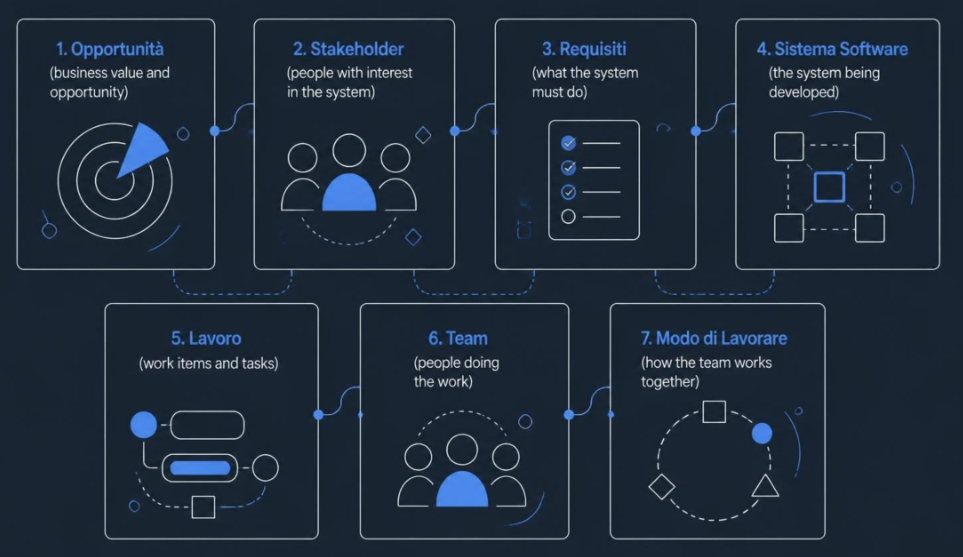
\includegraphics[width=0.88\textwidth]{7alpha.png}
     \caption{I 7 Alpha del Kernel di Essence e le tre Aree di Interesse.}
     \label{fig:essence_7_alpha}
\end{figure}

\begin{itemize}
    \item Kernel tradotto in mazzi di carte
    \item Milestone mapping: quali stati di quali Alpha servono per un traguardo
    \item Checkpoint: audit periodici tramite checklist degli stati
    \item Legame tra Alpha e stati: impossibile work ``under control'' ma team solo ``formed''
\end{itemize}
Project Health = evidenze dei checkpoint; chasing the state: isolare i checkpoint scoperti del prossimo stato, raccogliere evidenze mancanti e rivalutare.\\

\noindent Dimensioni di una pratica
\begin{enumerate}
    \item \textbf{Obiettivo}: il valore che la pratica persegue.
    \item \textbf{Alpha di interesse}: Alpha su cui interviene.
    \item \textbf{Work Products}: artefatti prodotti o usati come evidenza.
    \item \textbf{Attività}: compiti da svolgere.
    \item \textbf{Competenze}: abilità minime necessarie.
    \item \textbf{Criteri di avanzamento}: entry ed exit criteria.
    \item \textbf{Pattern ed esempi}: modelli e convenzioni riutilizzabili.
    \item \textbf{Supporti ausiliari}: strumenti, AI, vincoli di sicurezza.
\end{enumerate}

\noindent Esempio: code review con essence:
\begin{itemize}
    \item \textbf{Purpose}: valutare modifiche prima dell'integrazione e condividere conoscenza
    \item \textbf{Alpha primario}: software system + team e way of working in supporto
    \item \textbf{Work product}: review record strutturato
    \item \textbf{Attività}: preparare review, examine change, resolve findings, confirm integration
    \item \textbf{Competenze}: development, testing, comprensione del sistema, comunicazione costruttiva
    \item \textbf{LLM}: supporto alla review + verifica umana
\end{itemize}

\section{Processi agili}
I quattro pilastri:
\begin{enumerate}
    \item Individui e interazioni > processi e strumenti
    \item Software funzionante > documentazione
    \item Collaborazione con il cliente > negoziazione contrattuale
    \item Rispondere al cambiamento > piano prefissato
\end{enumerate}

\noindent Una fase per volta: \textbf{in uno Sprint il team fa sia requisiti, design, codice e test}.\\

\noindent Ruoli:
\begin{itemize}
    \item \textbf{Pig}: Product Owner, Scrum Master e Dev Team
    \item \textbf{Chicken}: stakeholder esterni
\end{itemize}

\noindent Scrum Team:
\begin{itemize}
    \item \textbf{Product Owner} (PO): interessi del committente e utenti finali. Visione, valore economico, ordina proprietà Product Backlog, date di scadenza. Ponte tra team tecnico e stakeholder
    \item \textbf{Srum Master} (SM): supporta, facilita meeting e cerimonie, rimuove ostacoli operativi, protegge da interruzioni, organizzazione
    \item \textbf{Dev Team} (DT): auto-organizzato, cross-funzionale, t-shaped (competenza primaria + conoscenze trasversali per ogni dev), tempo pieno
\end{itemize}

\noindent Controllo Empirico:
\begin{itemize}
    \item Trasparenza: pigs ben definiti, DoD\footnote{Codifica comletata, unit tests ok, test d'integrazione ok, test sicurezza ok, doc aggiornata.}
    \item Ispezione: software esaminato regolarmente, NO pesantezza burocratica
    \item Adattamento: if anomalie then team corregge rotta subito
\end{itemize}

\paragraph{1. Product Backlog} Elenco ordinato e dinamico di tutto ciò che potrebbe essere necessario nel prodotto. Lo gestisce SOLO il PO ed è composto da PBI (Product Backlog Items). Si divide in:
\begin{itemize}
    \item \textbf{Features}
    \item \textbf{Bugs}
    \item \textbf{Lavoro tecnico}: interventi su arch/server/migrations
    \item \textbf{Knowledge acquisition}: ricerca, POC, studi su fattibilità
\end{itemize}

\paragraph{2. Sprint} Unità base di 1-4 settimane che include \textbf{tutte le attività} (analisi, progettazione, codifica e collaudo). Ogni sprint deve avere un \textbf{incremento di MVP}.\\
\begin{center}
    \textit{No change during sprint.}
\end{center}

\noindent Sprint planning (1h $\cdot$ settimane durata sprint):
\begin{itemize}
    \item Fase ``What'': si def lo \textbf{Sprint Goal}\footnote{Lo sprint goal è una breve dichiarazione che sintetizza l'impatto della Sprint, fornendo al team una direzione.} e si selezionano le storie (DoR)\footnote{Comprensione da parte di tutti, dettagliata abbastanza, chiaro valore finale, stimabile in effort, indipendente da blocchi esterni.}
    \item Fase ``How'': si scompongono le storie in \textbf{task} e si forma \textbf{Sprint Backlog} con l'effort stimato per ogni task (in ore lavorative)
\end{itemize}

\noindent Flusso:
\begin{center}
    Story $\rightarrow$ To do $\rightarrow$ In progress $\rightarrow$ Review/test $\rightarrow$ Done
\end{center}

\paragraph{3. Daily Scrum} stand up meeting \textbf{riservato ai devs}. NO problem solving, rispondi a ``Cos'ho fatto ieri per progredire?'', ``Cosa farò oggi?'', ``Quali ostacoli mi stanno rallentando?''

\paragraph{4. Burndown chart e Team Velocity} Relazione tra effort residuo e tempo trascorso.

\paragraph{5. Sprint Review} Incontro di chiusura della sprint. Dimostrazione \textbf{live (no slides)} del software funzionante, verifica backlog e feedback immediato.

\paragraph{6. Sprint Retrospective} Sessione interna per esaminazione di relazioni personali, metodologie e strumenti tecnici. Formato \textbf{Start, Stop, Continue} (cosa iniziare a fare, cosa smettere di fare, cosa continuare a fare)

\paragraph{7. Product Backlog Refinement} PO e Dev Team fanno manutenzione del backlog (scomporre storie ampie, update efforts, acceptance criteria, priorità)

\paragraph{User stories}
\begin{center}
    (Ruolo) As a ... \\
    (Scopo) I want ... \\
    (Valore) so that ...
\end{center}
\textbf{User Stories $\neq$ Task (tecnici)}\\

\noindent \textbf{Vertical Slicing > Horizontal Slicing}: esempio della torta (fetta intera, non prima la panna, poi la crema, ...)\\

\noindent User Stories come frammenti di una conversazione continua: convergenza di tutte le figure professionali attorno alla stessa user story.\\

\noindent \textbf{INVEST}
\begin{itemize}
    \item Independent
    \item Negotiable
    \item Valuable
    \item Estimable
    \item Sized right
    \item Testable
\end{itemize}

\noindent Le user stories vengono stimate in \textbf{Story Points}


\paragraph{MVP} Funge da:
\begin{itemize}
    \item Verifica di ipotesi
    \item Criterio di decisione
\end{itemize}
Minimum = minor tempo possibile; Viable = esperienza d'uso sufficientemente completa.

\paragraph{Testing} Debugging non basta $\rightarrow$ testing automatico (70\% dei test)
\begin{itemize}
    \item Unit testing: test di singole unità software (automatizzato, facile da implementare e da eseguire, rapido, parte del progetto)
    \item Ciclo: obiettivo --- codice di test --- esecuzione test --- debug if red
\end{itemize}

\noindent TDD: ciclo \textbf{Red-Green-Refactor}\\

\noindent \textbf{CI (Continuous Integration)}: confluire proprie modifiche nel main trunk
\begin{itemize}
    \item Verifica automatica immediata
    \item Visibilità e correzione del guasto
    \item Minimizzare divergenze
\end{itemize}

\noindent YAGNI, tecnica del pomodoro e Pair Programming.

\newpage

\subsection{La qualità del software}
Non è unica e oggettiva, è il grado in cui il prodotto soddisfa i bisogni dei suoi stakeholder. La qualità è \textbf{dipendente} dal soggetto e \textbf{multidimensionale}.\\

\begin{itemize}
    \item \textbf{Errore}: azione umaana sbagliata (interpretazione errata della specifica)
    \item \textbf{Difetto (bug)}: imperfezione nel codice/in un documento
    \item \textbf{Guasto (failure)}: comportamento osservabile non previsto dalla specifica
\end{itemize}
Non tutti i difetti pesano uguale.\\

\noindent La qualità si può osservare a quattro livelli legati da una catena di influenza:
\begin{center}
\begin{tikzpicture}[
    font=\scriptsize\sffamily,
    box/.style={draw, rounded corners=3pt, text width=2.9cm, minimum height=1.5cm, align=center, fill=orange!5},
    ar/.style={-{Stealth[scale=0.9]}}
]
    \node[box] (proc) {\textbf{Qualità del processo}\\ come sviluppiamo\\ \textit{es. \% di codice revisionato}};
    \node[box, right=1.1cm of proc] (int) {\textbf{Qualità interna}\\ visibile a chi costruisce\\ \textit{es. complessità, duplicazione}};
    \node[box, right=1.1cm of int] (ext) {\textbf{Qualità esterna}\\ visibile eseguendo il sistema\\ \textit{es. tempo di risposta, guasti}};
    \node[box, right=1.1cm of ext] (use) {\textbf{Qualità in uso}\\ nel contesto reale\\ \textit{es. efficacia, soddisfazione}};
    \draw[ar] (proc) -- node[above, font=\tiny]{influenza} (int);
    \draw[ar] (int) -- node[above, font=\tiny]{influenza} (ext);
    \draw[ar] (ext) -- node[above, font=\tiny]{influenza} (use);
\end{tikzpicture}
\end{center}

\begin{itemize}
    \item Qualità \textbf{interna}: misurata senza eseguire codice
    \item Qualità \textbf{esterna}: misurata eseguendo codice
    \item Qualità \textbf{in uso}: misurata con utenti reali
\end{itemize}

\noindent \textit{\underline{ISO/IEC 25010:2023}}: il modello di qualità del prodotto:
\begin{center}
\small
\begin{tabular}{p{3.4cm}p{9.6cm}p{3.0cm}}
    \toprule
    \textbf{Caratteristica} & \textbf{Sottocaratteristiche e significato} & \textbf{Note 2023} \\
    \midrule
    \textbf{Idoneità funzionale} & Completezza, correttezza: il prodotto fornisce le funzioni richieste con risultati corretti. & \\
    \addlinespace
    \textbf{Efficienza prestazionale} & Tempi di risposta, utilizzo delle risorse, capacità: il prodotto è rapido ed efficiente nelle condizioni dichiarate. & \\
    \addlinespace
    \textbf{Compatibilità} & Coesistenza, interoperabilità: il prodotto convive con altri sistemi e scambia informazioni con essi. & \\
    \addlinespace
    \textbf{Capacità di interazione} & Riconoscimento, apprendimento, operabilità, protezione dagli errori, estetica, accessibilità. & ex \textit{usabilità} \\
    \addlinespace
    \textbf{Affidabilità} & Disponibilità, tolleranza ai guasti, recuperabilità: il prodotto opera senza interruzioni e si riprende dagli errori. & \\
    \addlinespace
    \textbf{Security} & Riservatezza, integrità, non ripudio, responsabilità, autenticità: il prodotto protegge dati e accessi. & \\
    \addlinespace
    \textbf{Manutenibilità} & Modularità, riusabilità, analizzabilità, modificabilità, testabilità: il prodotto si può comprendere, correggere ed evolvere. & \\
    \addlinespace
    \textbf{Flessibilità} & Adattabilità, installabilità, sostituibilità: il prodotto si adatta a contesti e piattaforme diverse. & ex \textit{portabilità} \\
    \addlinespace
    \textbf{Safety} & Assenza di rischi inaccettabili per persone, beni e ambiente durante l'uso del sistema. & nuova nel 2023 \\
    \bottomrule
\end{tabular}
\end{center}

\paragraph{Cosa si misura} Tre famiglie:
\begin{center}
\small
\begin{tabular}{p{5.2cm}p{5.2cm}p{5.2cm}}
    \toprule
    \textbf{Risorse} & \textbf{Processo} & \textbf{Prodotto} \\
    \midrule
    tempo, sforzo, costi & come lavoriamo & cosa abbiamo costruito \\
    \addlinespace
    mesi-persona; costo preventivo vs consuntivo; livelli di staff & \% difetti trovati per fase; \textit{cycle time}, \textit{velocity}; stabilità dei requisiti & LOC, \textit{function point}; complessità ciclomatica; copertura, difetti per KLOC \\
    \bottomrule
\end{tabular}
\end{center}

\begin{itemize}
    \item Dev: guarda copertura e difetti dei propri test
    \item Team: guarda stato dei requisiti, test superati e difetti aperti
    \item Org: guarda difetti rilasciati per gravità e accuratezza delle stime
\end{itemize}

\paragraph{Complessità ciclomatica} Misura il numero di cammini linearmente indipendenti nel grafo di controllo di un programma:
\[
V(G) = ARCHI-NODI+2
\]

\paragraph{Goal-Question-Metric} Lega la misura agli obiettivi:
\begin{center}
\small
\begin{tabular}{p{2.4cm}p{5.4cm}p{8.0cm}}
    \toprule
    \textbf{Livello} & \textbf{Domanda guida} & \textbf{Esempio} \\
    \midrule
    \textbf{Goal} & Perché misuriamo? & Valutare l'affidabilità del prodotto. \\
    \addlinespace
    \textbf{Question} & Che cosa ci serve sapere? & Qual è la distribuzione dei guasti? Il codice rispetta lo standard? Le revisioni sono efficaci? \\
    \addlinespace
    \textbf{Metric} & Che dato raccogliamo? & Numero di guasti per modulo; violazioni per modulo; difetti trovati in revisione. \\
    \bottomrule
\end{tabular}
\end{center}

\begin{itemize}
    \item \textbf{G}: alla relazione finale devono contribuire tutti i membri del gruppo.
    \item \textbf{Q1}: quante ore ha lavorato ciascuno? \quad \textbf{M1}: ore registrate da ciascun membro.
    \item \textbf{Q2}: quanta parte della relazione ha scritto ciascuno? \quad \textbf{M2}: percentuale di sezioni o di commit per autore.
\end{itemize}

\paragraph{Verifica e Testing}
\begin{itemize}
    \item Verifica: ``stiamo costruendo il prodotto nel modo giusto?''. Riguarda la conformità alla specifica e alle decisioni. Si attua con ispezioni, analisi del codice e test
    \item Validazione: ``stiamo costruendo il progetto giusto?''. Riguarda l'accettazione del committente e il soddisfacimento di un bisogno reale. Si attua con test di accettazione, dimostrazioni e uso controllato.
\end{itemize}

\begin{center}
\small
\begin{tabular}{p{4.2cm}p{5.2cm}p{6.4cm}}
    \toprule
    \textbf{Livello di specifica} & \textbf{Test corrispondente} & \textbf{Che cosa si verifica} \\
    \midrule
    Requisiti & Test di accettazione & Conformità al bisogno del committente (validazione). \\
    \addlinespace
    Architettura & Test di sistema & Comportamento dell'intero sistema rispetto ai requisiti. \\
    \addlinespace
    Progetto dei moduli & Test di integrazione & Interfacce, contratti e collaborazione tra componenti. \\
    \addlinespace
    Codice & Test di unità & Correttezza delle singole unità (funzioni, classi, metodi). \\
    \bottomrule
\end{tabular}
\end{center}

\begin{center}
\begin{tikzpicture}[font=\scriptsize\sffamily]
    \node[draw, fill=orange!25, minimum width=3.4cm, minimum height=0.8cm] (e2e) at (0,2.4) {End-to-end e accettazione};
    \node[draw, fill=orange!15, minimum width=6.8cm, minimum height=0.9cm] (int) at (0,1.1) {Integrazione e sistema};
    \node[draw, fill=orange!7, minimum width=10.2cm, minimum height=1.0cm] (unit) at (0,-0.2) {Unità};
    \node[font=\tiny, align=left, anchor=west] at (5.4,2.4) {pochi, lenti, fragili\\ Selenium, Playwright};
    \node[font=\tiny, align=left, anchor=west] at (5.4,1.1) {interfacce tra componenti\\ Testcontainers, API test};
    \node[font=\tiny, align=left, anchor=west] at (5.4,-0.2) {molti, veloci, economici\\ JUnit, pytest};
\end{tikzpicture}
\end{center}

Le tecniche di test si distinguono per il tipo di informazione utilizzata:

\begin{center}
\small
\begin{tabular}{p{7.2cm}p{7.2cm}}
    \toprule
    \textbf{Black-box (funzionale)} & \textbf{White-box (strutturale)} \\
    \midrule
    Deriva dalla \textbf{specifica}: il codice è trattato come una scatola nera. & Deriva dal \textbf{codice sorgente}: la struttura interna guida la scelta dei casi. \\
    \addlinespace
    Classi di equivalenza, valori limite, tabelle di decisione, test basati sui casi d'uso. & Copertura dei comandi, delle decisioni e dei cammini; \textit{mutation testing}. \\
    \addlinespace
    Verifica il comportamento osservabile rispetto ai requisiti. & Verifica l'esecuzione effettiva delle parti del programma. \\
    \bottomrule
\end{tabular}
\end{center}

\begin{itemize}
    \item Analisi statica: esamina codice e dipendenze + ricerca statica di bug e vulnerabilità senza eseguire codice
    \item Quality gate: insieme di soglie oggettive da superare
\end{itemize}
Nella pipeline:
\begin{center}
\begin{tikzpicture}[
    font=\tiny\sffamily,
    st/.style={draw, rounded corners=2pt, text width=1.95cm, minimum height=0.85cm, align=center, fill=orange!7},
    ar/.style={-{Stealth[scale=0.8]}}
]
    \node[st] (c) {Commit\\ push o PR};
    \node[st, right=0.18cm of c] (b) {Build\\ compilazione};
    \node[st, right=0.18cm of b] (t) {Test\\ unità e integrazione};
    \node[st, right=0.18cm of t] (s) {Analisi statica\\ bug, vulnerabilità, smell};
    \node[st, right=0.18cm of s] (q) {Quality gate\\ soglie superate?};
    \node[st, right=0.18cm of q] (r) {Rilascio\\ deploy};
    \draw[ar] (c) -- (b);
    \draw[ar] (b) -- (t);
    \draw[ar] (t) -- (s);
    \draw[ar] (s) -- (q);
    \draw[ar] (q) -- (r);
\end{tikzpicture}
\end{center}

\noindent SonarQube è uno degli strumenti per l'analisi statica. Può operare nell'IDE, nella pipeline CI, nella PR. Controlla:
\begin{itemize}
    \item Affidabilità
    \item Sicurezza
    \item Manutenibilità
\end{itemize}
Calcola un rapporto di debito:
\[
\text{rapporto di debito} = \frac{\text{debito tecnico}}{30 \text{ min } \cdot \text{ righe di codice}}
\]
\begin{center}
\small
\begin{tabular}{p{2.0cm}p{2.4cm}p{2.4cm}p{2.4cm}p{2.4cm}p{2.4cm}}
    \toprule
    \textbf{Rating} & \textbf{A} & \textbf{B} & \textbf{C} & \textbf{D} & \textbf{E} \\
    \midrule
    Rapporto di debito & $\le 5\%$ & $<10\%$ & $<20\%$ & $<50\%$ & $\ge 50\%$ \\
    \bottomrule
\end{tabular}
\end{center}

\subsection{Le forme dei requisiti}
\paragraph{Cosa sono i requisiti}
La forma giusta dipende dal lettore. Definizioni:
\begin{itemize}
    \item Vocabolario: ``Ciascuna delle qualità necessarie e richieste per uno scopo determinato''
    \item \textbf{IEEE 610.12-1990}: distingue due oggetti:
    \begin{itemize}
        \item \textbf{bisogno}: condizione/capacità necessaria ad un \underline{utente} per risolvere un problema/raggiungere un obiettivo
        \item \textbf{impegno}: condizione/capacità che un \underline{sistema} deve possedere per soddisfare contratto/standard/spec
    \end{itemize} 
\end{itemize}

\noindent Legge di Humphrey: 
\begin{itemize}
    \item ``I requisiti non saranno chiari finché gli utenti non inizieranno a usarlo.'' (IKIWISI: `I'll know it when I see it')
    \item ``Un problema non è ben compreso finché non si sviluppa una soluzione''.
    \item Quindi: i requisiti \textbf{emergono per iterazioni}
\end{itemize}

\noindent Tipi di requisito:
\begin{itemize}
    \item \textbf{Funzionale}: cosa deve fare il sistema
    \item \textbf{Di qualità}: quanto bene lo fa (misurabile)
    \item \textbf{Vincolo}: limite su come o dove si realizza
\end{itemize}

\noindent Misurabilità dei requisiti con norma ISO/IEC 25010:2023 (modello di qualità del prodotto)
\begin{center}
\small
\begin{tabular}{p{3.0cm}p{4.6cm}p{7.6cm}}
    \toprule
    \textbf{Caratteristica} & \textbf{Requisito vago} & \textbf{Requisito misurabile} \\
    \midrule
    \textbf{Efficienza prestazionale} & ``La ricerca deve essere veloce'' & Con 100.000 volumi e 200 utenti contemporanei, il 95\% delle ricerche risponde in meno di 1 s. \\
    \addlinespace
    \textbf{Capacità di interazione} & ``L'app deve essere facile'' & Un nuovo iscritto completa il primo prestito senza aiuto in meno di 3 minuti (test con 10 utenti: almeno 9 ci riescono). \\
    \addlinespace
    \textbf{Affidabilità} & ``Il sistema deve funzionare sempre'' & Disponibilità $\geq 99{,}5\%$ nell'orario di apertura, misurata su base mensile. \\
    \addlinespace
    \textbf{Security} & ``I dati devono essere protetti'' & Le operazioni del bibliotecario richiedono autenticazione a due fattori; ogni accesso ai dati personali è registrato. \\
    \bottomrule
\end{tabular}
\end{center}

\noindent Formula del requisito verificabile:
\begin{center}
    \textbf{metrica + soglia + condizioni di misura} = requisito verificabile
\end{center}

\noindent Livelli dei requisiti:
\begin{center}
\small
\begin{tabular}{p{2.0cm}p{5.2cm}p{8.0cm}}
    \toprule
    \textbf{Livello} & \textbf{Domanda e documenti} & \textbf{Esempio: biglietteria} \\
    \midrule
    \textbf{Business} & Perché serve il prodotto? Visione. & Ridurre le code in biglietteria: entro un anno almeno metà dei biglietti venduti online. \\
    \addlinespace
    \textbf{Utente} & Chi lo userà e cosa ci farà? Casi d'uso, user story. & Come viaggiatore voglio comprare un biglietto Bologna--Milano dal telefono. \\
    \addlinespace
    \textbf{Software} & Cosa dovrà fare il sistema? Specifica (SRS), criteri di accettazione. & Per ogni acquisto confermato, il sistema emette un biglietto con tratta, data, passeggero e codice univoco. \\
    \bottomrule
\end{tabular}
\end{center}

\noindent \underline{Distinzione tra \textbf{requisito} (scopo) e \textbf{scelta di progetto} (soluzione)}
\begin{center}
\small
\begin{tabular}{p{7.4cm}p{7.4cm}}
    \toprule
    \textbf{Requisito (scopo)} & \textbf{Scelta di progetto (soluzione)} \\
    \midrule
    L'iscritto prenota un volume già in prestito & Una tabella \texttt{Prenotazioni} con chiave ISBN \\
    \addlinespace
    L'iscritto viene avvisato quando il volume rientra & Notifiche push tramite Firebase \\
    \addlinespace
    Il bibliotecario vede i prestiti scaduti & Una vista SQL aggiornata ogni notte \\
    \addlinespace
    La ricerca risponde in meno di 1 secondo & Un indice full-text Elasticsearch \\
    \bottomrule
\end{tabular}
\end{center}

\paragraph{Le forme classiche} Lo stesso bisogno può essere espresso in forme diverse. Per esempio, Paolo deve arrivare puntuale da qualche parte e ha bisogno di un taxi in via X. Tre modi per descriverlo:
\begin{itemize}
    \item \textbf{requisito funzionale}: ``Il sistema permetterà di prenotare un taxi e di ottenere una stima del tempo di attesa''.
    \item \textbf{scenario}: ``Fragola33 arriverà tra 5 minuti''
    \item \textbf{user story}: ``Come Paolo voglio chiamare un taxi dall'app e sapere quando arriverà, per capire se sarò puntuale all'appuntamento''.
\end{itemize}

\newpage

\begin{center}
\small
\begin{tabular}{p{4.2cm}p{5.6cm}p{5.4cm}}
    \toprule
    \textbf{Lettore} & \textbf{Forme tipiche} & \textbf{Scopo} \\
    \midrule
    Cliente e utenti & User story, job story, personae & Condividere bisogno e valore. \\
    \addlinespace
    Chi progetta l'interazione & Casi d'uso, scenari, storyboard & Descrivere flussi ed eccezioni. \\
    \addlinespace
    Contratto e certificazione & Documento SRS, frasi ``il sistema deve\ldots'' & Fissare impegni tracciabili. \\
    \addlinespace
    Sviluppatori e tester & Criteri di accettazione, Gherkin, modelli & Rendere il comportamento verificabile. \\
    \addlinespace
    LLM che genera codice & Specifiche strutturate: EARS, Gherkin, modelli di dominio & Ridurre le interpretazioni arbitrarie. \\
    \bottomrule
\end{tabular}
\end{center}

\begin{figure}[htbp]
    \centering
    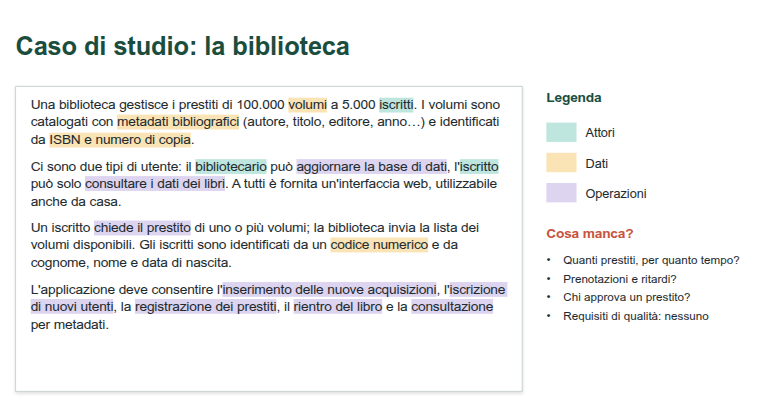
\includegraphics[width=0.75\textwidth]{biblioteca.png}
\end{figure}

\noindent I requisiti della biblioteca in forma funzionale:
\begin{center}
\small
\begin{tabular}{p{0.9cm}p{9.6cm}p{4.7cm}}
    \toprule
    \textbf{ID} & \textbf{Requisito} & \textbf{Note del revisore} \\
    \midrule
    R1 & Il sistema gestirà due tipi di utenti: bibliotecario e iscritto & \\
    R2 & Il sistema permetterà all'iscritto di ottenere un libro in prestito & Perché? Per quanto tempo? Quanti volumi? \\
    R3 & Il sistema permetterà all'iscritto di restituire un libro & \\
    R4 & Il sistema permetterà al bibliotecario di inserire un nuovo libro nel catalogo & \\
    R5 & Il sistema permetterà al bibliotecario di dismettere un libro & \\
    R6 & Il sistema permetterà al bibliotecario di iscrivere un nuovo utente & \\
    R7 & Il sistema permetterà al bibliotecario di sollecitare una restituzione & Quando si sollecita? Con quale mezzo? \\
    R8 & Il sistema permetterà al bibliotecario di elaborare statistiche sui prestiti & Quali statistiche, per chi? \\
    \midrule
    Tutti & Nessun criterio di accettazione & Come li collaudo? \\
    \bottomrule
\end{tabular}
\end{center}

\newpage
\noindent \textit{Osservazioni}:
\begin{enumerate}
    \item R5, R7, R8 \textbf{non sono nel testo del cliente} (sono emersi dal colloquio e vanno confermati)
    \item \textbf{nessun requisito ha un criterio di accettazione} (la forma funzionale dice ``cosa'' serve, non ``quando'' è soddisfatto)
\end{enumerate}

\noindent Use Case Diagram in UML:
\begin{figure}[htbp]
    \centering
    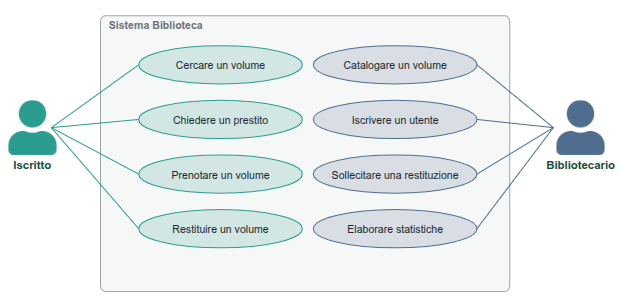
\includegraphics[width=0.75\textwidth]{usecase.png}
\end{figure}

\begin{figure}[htbp]
    \centering
    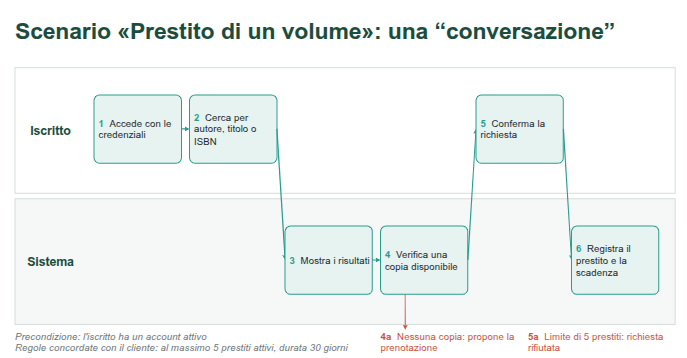
\includegraphics[width=1\textwidth]{scenario.png}
\end{figure}

\clearpage

\noindent Confronto tra le forme:
\begin{center}
\small
\begin{tabular}{p{3.2cm}p{4.4cm}p{3.6cm}p{4.0cm}}
    \toprule
    \textbf{Forma} & \textbf{Punti di forza} & \textbf{Limiti} & \textbf{Quando usarla} \\
    \midrule
    Documento SRS & Completo, contrattuale, tracciabile & Costoso da mantenere; può invecchiare in fretta & Appalti, sistemi critici \\
    \addlinespace
    Casi d'uso e scenari & Flussi ed eccezioni espliciti & Verbosi; poco centrati sul valore & Interazioni complesse \\
    \addlinespace
    User story & Valore e utente al centro; leggere & Ambigue senza conversazione & Backlog agile \\
    \addlinespace
    Prototipi e mockup & Mostrano invece di descrivere & Non dicono regole e dati & Interfacce, validazione precoce \\
    \addlinespace
    Gherkin / EARS & Strutturati, verificabili, testabili & Richiedono disciplina; non eliminano ogni ambiguità & Criteri di accettazione, input per l'IA \\
    \bottomrule
\end{tabular}
\end{center}

\noindent Una scelta ragionevole è \textbf{quali forme combinare}, non ``qual è LA forma''.

\paragraph{User story} Scompongono una visione in elementi abbastanza piccoli da essere realizzati in una sprint. Gerarchia:
\begin{center}
    Visione $\rightarrow$ Epiche $\rightarrow$ User stories
\end{center}
Un'epica è troppo grande per uno Sprint.\\

\noindent Modelli:
\begin{center}
\small
\begin{tabular}{p{7.4cm}p{7.4cm}}
    \toprule
    \textbf{Connextra: centrata sul ruolo} & \textbf{Job story: centrata sulla situazione} \\
    \midrule
    Come \textit{<ruolo>} voglio \textit{<funzione>} per \textit{<beneficio>} & Quando \textit{<situazione>} voglio poter \textit{<azione>} così da \textit{<risultato>} \\
    \addlinespace
    ``Come iscritto voglio prenotare un volume in prestito per averlo appena rientra'' & ``Quando ho bisogno di un libro già in prestito, voglio poterlo prenotare, così da averlo appena rientra'' \\
    \bottomrule
\end{tabular}
\end{center}

\newpage

\noindent Le storie si ricavano da \textbf{personae}:
\begin{center}
    interviste e dati $\rightarrow$ schemi ricorrenti $\rightarrow$ persona $\rightarrow$ user story
\end{center}

\noindent Una US da sola è solo la Card:
\begin{figure}[htbp]
    \centering
    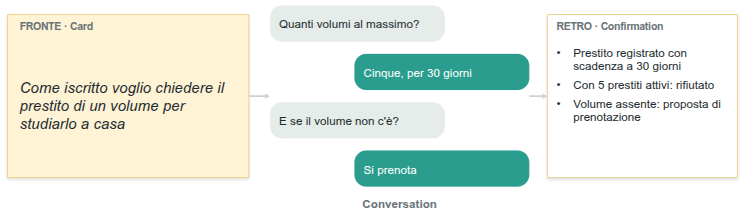
\includegraphics[width=0.75\textwidth]{3C.png}
\end{figure}

\noindent I criteri di accettazione si possono scrivere in Gherkin, lo scenario diventa un file \texttt{.feature}:
\begin{lstlisting}
Scenario: limite di prestiti raggiunto
  Given un iscritto con 5 prestiti attivi
  When chiede il prestito di un altro volume
  Then la richiesta viene rifiutata
  And vede il messaggio "Limite di 5 prestiti raggiunto"
\end{lstlisting}
Ogni passo è una step definition, in Python:
\begin{lstlisting}[language=Python]
@given("un iscritto con 5 prestiti attivi", target_fixture="iscritto")
def iscritto(): return Iscritto(prestiti=5)

@when("chiede il prestito di un altro volume", target_fixture="esito")
def richiesta(iscritto): return presta(iscritto)

@then("la richiesta viene rifiutata")
def rifiutata(esito): assert not esito.ok
\end{lstlisting}

\noindent Una buona storia rispetta INVEST:
\begin{center}
\small
\begin{tabular}{p{2.4cm}p{6.2cm}p{6.6cm}}
    \toprule
    \textbf{Criterio} & \textbf{Storia debole} & \textbf{Storia migliorata} \\
    \midrule
    \textbf{I}ndipendente & $\times$ tocca tutto il sistema & ? dipende da prestito e prenotazione \\
    \addlinespace
    \textbf{N}egoziabile & \checkmark\ ma solo perché è vaga & \checkmark\ i dettagli si discutono \\
    \addlinespace
    \textbf{V}alore & $\times$ non dice per chi né perché & \checkmark\ l'iscritto evita una visita in biblioteca \\
    \addlinespace
    \textbf{E}stimabile & $\times$ ``efficiente'' non si stima & ? perimetro chiaro; stimano gli sviluppatori \\
    \addlinespace
    \textbf{S}piccola & $\times$ troppo ampia: va scomposta & ? forse sta in uno Sprint: lo valuta il team \\
    \addlinespace
    \textbf{T}estabile & $\times$ nessun criterio di accettazione & \checkmark\ criterio: rinnovo rifiutato se prenotato \\
    \bottomrule
\end{tabular}
\end{center}

\newpage

\begin{figure}[htbp]
    \centering
    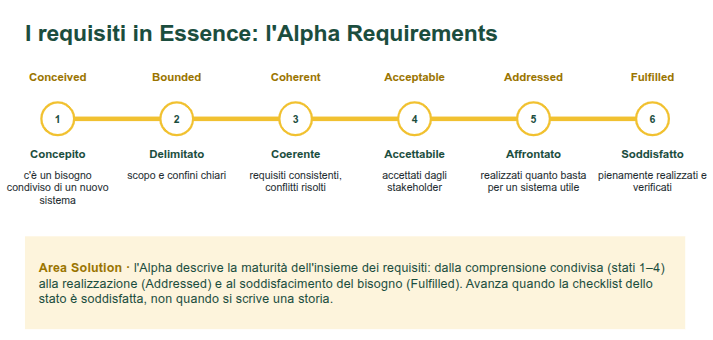
\includegraphics[width=0.75\textwidth]{essence.png}
\end{figure}

\paragraph{LLM} Vanno trattati come programmatori in coppia molto letterali: vibe-coding vs Prompt con US vs \textbf{Spec-Driven Development}, fatto da quattro fasi:
\begin{itemize}
    \item \textbf{Specify}: cosa e perché; criteri di successo (\texttt{requirements.md}: US e criteri in EARS)
    \item \textbf{Plan}: architettura, tecnologie e vincoli (\texttt{design.md}: architettura e sequence diagrams)
    \item \textbf{Tasks}: compiti piccoli e verificabili (\texttt{tasks.md})
    \item \textbf{Implement}: realizzazione e review umana
\end{itemize}

\noindent EARS (Easy Approach to Requirements Syntax):
\begin{center}
\small
\begin{tabular}{p{2.4cm}p{5.4cm}p{7.4cm}}
    \toprule
    \textbf{Schema} & \textbf{Forma} & \textbf{Esempio: biblioteca} \\
    \midrule
    \textbf{Ubiquo} & Il \textit{<sistema>} deve \textit{<risposta>} & Il sistema deve identificare ogni copia con ISBN e numero di copia. \\
    \addlinespace
    \textbf{Evento} & Quando \textit{<evento>}, il \textit{<sistema>} deve\ldots & Quando un volume rientra, il sistema deve avvisare il primo iscritto in prenotazione. \\
    \addlinespace
    \textbf{Stato} & Mentre \textit{<stato>}, il \textit{<sistema>} deve\ldots & Mentre un iscritto ha un prestito scaduto, il sistema deve impedirgli nuovi prestiti. \\
    \addlinespace
    \textbf{Indesiderato} & Se \textit{<condizione>}, allora il \textit{<sistema>} deve\ldots & Se un iscritto con 5 prestiti attivi chiede un altro prestito, allora il sistema deve rifiutarlo. \\
    \addlinespace
    \textbf{Opzione} & Dove \textit{<funzione presente>}, il \textit{<sistema>} deve\ldots & Dove è attivo il prestito digitale, il sistema deve fornire il link all'e-book. \\
    \bottomrule
\end{tabular}
\end{center}

\begin{lstlisting}[language=Python]
## Storia
Come iscritto voglio un volume in prestito per studiare a casa

## Criteri (EARS)
Quando l`iscritto conferma e una copia risulta disponibile, il
sistema deve registrare il prestito con scadenza a 30 giorni.
Se l`iscritto ha 5 prestiti attivi, allora il sistema deve
rifiutare la richiesta.

## Modello di dominio
Iscritto(id, nome) . Copia(isbn, n, disponibile)
Prestito(iscritto, copia, inizio, scadenza)

## Requisiti non funzionali
Ricerca: 95% < 1 s con 100.000 volumi e 200 utenti
Dati personali (GDPR): quali e per quanto? -> chiedere al PO

## Istruzioni
Prima del codice, elenca i dubbi e le domande per il PO.
Non aggiungere funzioni non richieste.
\end{lstlisting}



\newpage

\section{UML}
\paragraph{Introduzione}
\begin{itemize}
    \item \textbf{Information hiding}: un modulo deve celare la propria implementazione interna ed esporsi tramite interfaccia pubblica (lettura e manipolazione dello stato tramite \textbf{accessor methods})
    \item \textbf{Coupling}: legame di dipendenza tra due moduli. Obiettivo = loose coupling (poche dip.)
    \item \textbf{Cohesion}: modulo i cui elementi sono atti allo svolgimento di un singolo e ben definito compito
\end{itemize}

\noindent Fasi di sviluppo:
\begin{itemize}
    \item \textbf{OO Concept Modeling}
    \item \textbf{OO Analysis}
    \item \textbf{OO Design}
    \item \textbf{OO Programming}
\end{itemize}

\noindent Concetti:
\begin{itemize}
    \item \textbf{Classe}: template astratto con \textbf{attributi} e \textbf{metodi}
    \item \textbf{Oggetto}: istanza concreta di una classe
    \item \textbf{Messaggi}: gli oggetti collaborano per message passing
    \item \textbf{Operazione/Service}: procedura eseguibile incapsulata all'interno di una classe
\end{itemize}

\begin{center}
    ``\textit{Il processo è a spirale, non verticale}''
\end{center}

\begin{figure}[htbp]
    \centering
    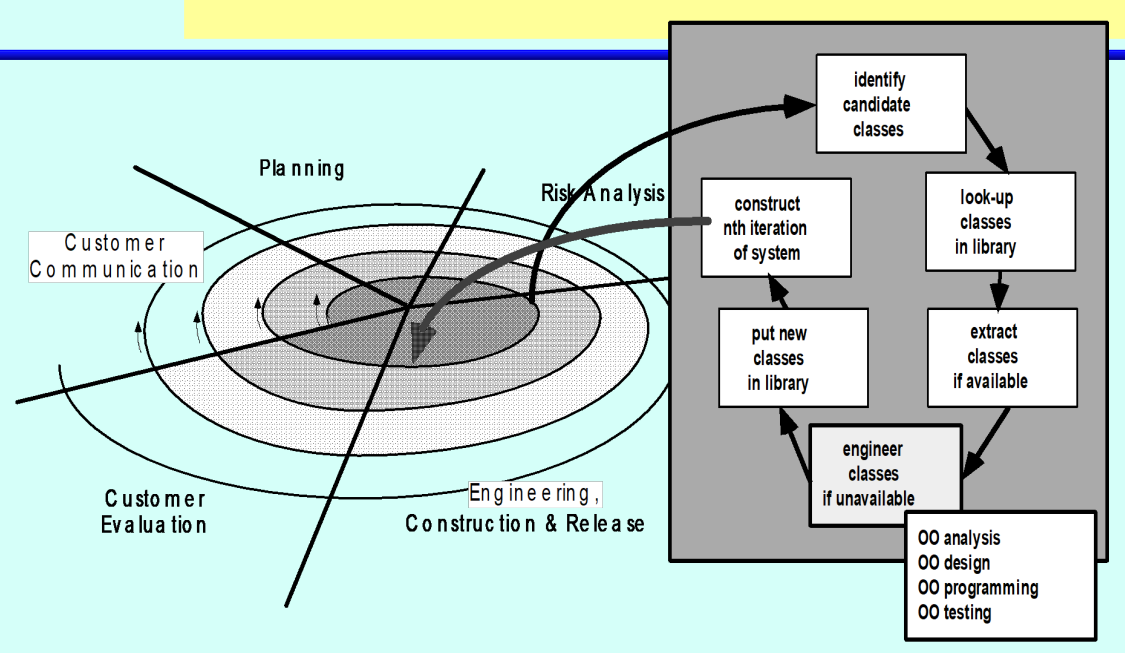
\includegraphics[width=0.75\textwidth]{spirale.png}
    \label{fig:spiral_oo_process}
\end{figure}

\noindent L'\textbf{ereditarietà} permette di define classi come estensioni di altre classi:
\begin{itemize}
    \item Relazione \textbf{is-a}: Dog is a Animal
    \item Relazione \textbf{extends}: estende le potenzialità della classe base
    \item Relazione \textbf{include}: Animals contiene concettualmente Dogs
    \item Relazione di \textbf{generalizzazione}: superclasse generalizza i tratti comuni condivisi da tutte le sotto-classi
\end{itemize}
Può essere \textbf{multipla}: una sottoclasse eredita contemporaneamente attributi e metodi da 2+ classi.\\

\noindent Il \textbf{polimorfismo} è la capacità di usare lo stesso nome per identificare metodi che fanno operazioni simili su oggetti di tipo differente:
\begin{itemize}
    \item \textbf{Overloading (polim. ad-hoc)}: stesso nome ma differiscono per lista di parametri (print(string) $\neq$ print(number))
    \item \textbf{Generico}: modello astratto definisce struttura/algoritmo comune ad un insieme di tipi (la funzione swap)
    \item \textbf{Overriding}: ridefinizione di un metodo all'interno di una classe derivata --- consente risoluzione dinamica a runtime
\end{itemize}

\subsection{OO Concept Modeling: Use Case Diagram} Ha fini di \textbf{Context Analysis} + \textbf{Requirement Analysis}. In UML corrisponde allo \textbf{Use Case Diagram} che ha relazioni tra casi d'uso di tipo:
\begin{itemize}
    \item \textbf{Relazione \texttt{<<includes>>}}: inclusione obbligatoria
    \item \textbf{Relazione \texttt{<<extends>>}}: comportamento opzionale che estende il caso d'uso base
\end{itemize}

\begin{figure}[htbp]
    \centering
\begin{tikzpicture}[
    font=\small\sffamily,
    usecase/.style={draw, ellipse, minimum width=3cm, minimum height=0.9cm, semithick, align=center},
    rel/.style={-{Stealth[scale=1]}, dashed, semithick, font=\scriptsize\sffamily}
]
    \actor{trader}{0}{0}{Trader}
    \node[usecase] (risk) at (4, 3) {Analyze risks};
    \node[usecase] (price) at (4, 0.8) {Price details};
    \node[usecase] (deal) at (4, -1.6) {Get the deal};
    \node[usecase] (limit) at (4, -4) {Limit exceeded};
    \node[usecase] (eval) at (9.2, 1.9) {Evaluation};
    \actor{sales}{9.2}{-2}{Sales system}

    \draw[semithick] (trader.east) -- (risk.west);
    \draw[semithick] (trader.east) -- (price.west);
    \draw[semithick] (trader.east) -- (deal.west);
    \draw[semithick] (sales.west) -- (price.east);
    \draw[semithick] (sales.west) -- (deal.east);

    \draw[rel] (risk.east) -- node[above, sloped] {\texttt{<<includes>>}} (eval.north west);
    \draw[rel] (price.east) -- node[below, sloped] {\texttt{<<includes>>}} (eval.south west);
    \draw[rel] (limit.north) -- node[right] {\texttt{<<extends>>}} (deal.south);
\end{tikzpicture}
    \label{fig:use_case_nyse_example}
\end{figure}

\noindent Questo diagramma è composto da \textbf{Attori} (ruolo assunto da entità esterna, come ``Trader'') e da \textbf{Use Cases} (come ``Price details'').\\

\noindent Al diagramma viene associata una descrizione testuale step-by-step o narrativa.\\

\noindent Nota:
\begin{figure}[htbp]
    \centering
\begin{tikzpicture}[font=\small\sffamily]
    \node[font=\footnotesize\bfseries\sffamily, text=red!70!black, anchor=west] at (-0.8, 4.3) {\guillemotleft\,ERRATO\,\guillemotright\ Anti-pattern ``The KILLER''};
    \actor{c1}{0}{0}{Customer}
    \sysbox{1.6}{-3.4}{13.4}{3.6}{Airline System}
    \node[ucase, draw=red!70!black, text=red!70!black, line width=1.1pt, minimum width=2.6cm, minimum height=1.2cm] (ui) at (4.2, 0) {System\\Main UI};
    \node[ucase] (s1) at (10.2, 2.4) {Reservation, schedule and fares};
    \node[ucase] (s2) at (10.2, 0.8) {Aeroplan frequent flyers};
    \node[ucase] (s3) at (10.2, -0.8) {Traveler services};
    \node[ucase] (s4) at (10.2, -2.4) {\dots};
    \draw[assoc] (c1.east) -- (ui.west);
    \foreach \n in {s1,s2,s3,s4} \draw[incl, red!70!black] (ui.east) -- node[above, sloped, pos=0.55, font=\tiny\sffamily] {\texttt{<<includes>>}} (\n.west);

    \begin{scope}[yshift=-8.6cm]
    \node[font=\footnotesize\bfseries\sffamily, text=green!40!black, anchor=west] at (-0.8, 4.3) {\guillemotleft\,CORRETTO\,\guillemotright\ Un caso d'uso per ogni obiettivo dell'utente};
    \actor{c2}{0}{0}{Customer}
    \sysbox{1.6}{-3.4}{13.4}{3.6}{Airline System}
    \node[ucase, draw=green!40!black, line width=1.1pt] (g1) at (7.5, 1.6) {Reserve Flight};
    \node[ucase, draw=green!40!black, line width=1.1pt] (g2) at (7.5, 0) {Check Miles Balance};
    \node[ucase, draw=green!40!black, line width=1.1pt] (g3) at (7.5, -1.6) {Update Address};
    \foreach \n in {g1,g2,g3} \draw[assoc] (c2.east) -- (\n.west);
    \end{scope}
\end{tikzpicture}
    \label{fig:the_killer_antipattern}
\end{figure}

\subsection{OO Analysis: Class Diagram} Lo scopo è comprendere a fondo il dominio del problema e formalizzarne i requisiti. Passi:
\begin{enumerate}
    \item Estrarre le classi
    \item Stabilirne le relazioni
    \item Definire la gerarchia
    \item Id attributi per ogni classe
    \item Id metodi per ogni classe
    \item Id relazioni tra classi e oggetti
    \item Costruire il modello comportamentale
    \item Iterare sui primi 5 passi
\end{enumerate}

\noindent Classe in UML (Nome, Attributi, Metodi/Operazioni):
\begin{figure}[htbp]
    \centering
\begin{tikzpicture}
    \node[cls, text width=5.2cm] {\cn{Task}\nodepart{second}startDate\\ endDate\nodepart{third}setStartDate(d : Date = default)\\ setEndDate(d : Date = default)\\ getDuration() : Date};
\end{tikzpicture}
    \label{fig:uml_class_box_example}
\end{figure}

\noindent Il \textbf{Class Diagram} definisce le seguenti relazioni (dalla più debole alla più forte):
\begin{itemize}
    \item \textbf{Dipendenza}: una classe impiega temporaneamente i servizi di un'altra
    \item \textbf{Associazione}: relazione semantica
    \item \textbf{Aggregazione}: relazione parte-tutto (``contiene/è composto da''). C'è sopravvivenza delle parti (esiste ancora ``Scaffale'' senza ``Libri'')
    \item \textbf{Composizione}: relazione parte-tutto \textbf{senza sopravvivenza} (non esiste ``Mazzo di fiori'' senza ``Fiori'')
    \item \textbf{Generalizzazione}: relazione is-a
\end{itemize}
Un'associazione può avere un nome, una direzione di lettura e molteplicità agli estremi:
\begin{figure}[htbp]
    \centering
\begin{tikzpicture}[cls/.append style={font=\small\sffamily}, lab/.style={font=\scriptsize\sffamily}]
    \node[cls, text width=3.4cm] (order) at (0, 0) {\cn{Order}\nodepart{second}dateReceived\\ isPrepaid\\ number : String\\ price : Money\nodepart{third}dispatch()};
    \node[cls, text width=3cm] (cust) at (8, 0) {\cn{Customer}\nodepart{second}name\\ address\nodepart{third}creditRating()};
    \draw[semithick] (order.east |- 0,0.3) -- node[lab, above] {hasCustomer $\blacktriangleright$} node[lab, pos=0.07, above] {$*$} node[lab, pos=0.93, above] {$1$} (cust.west |- 0,0.3);
\end{tikzpicture}
    \label{fig:association_order_customer}
\end{figure}

\begin{figure}[htbp]
    \centering
\begin{tikzpicture}[cls/.append style={font=\footnotesize\sffamily, text width=2.8cm}, lab/.style={font=\scriptsize\sffamily}]
    \node[font=\small\bfseries\sffamily] at (4.2, 2.2) {Associazione con ruoli bilaterali};
    \node[cls, rectangle split parts=2] (comp) at (0, 0) {\cn{Company}\nodepart{second}Name\\ Address};
    \node[cls, rectangle split parts=2] (pers) at (8.4, 0) {\cn{Person}\nodepart{second}Name\\ Insurance no.\\ Address};
    \draw[semithick] (comp.east |- 0,0.2) -- node[lab, above=7pt] {$\blacktriangleleft$ Works for} node[lab, pos=0.02, below, anchor=north west] {employer} node[lab, pos=0.98, below, anchor=north east] {employee} node[lab, pos=0.98, above, anchor=south east] {$*$} (pers.west |- 0,0.2);

    \begin{scope}[yshift=-5.6cm]
    \node[font=\small\bfseries\sffamily] at (4.2, 2.4) {Associazione riflessiva (ruoli obbligatori)};
    \node[cls, rectangle split parts=2] (p) at (3.2, 0) {\cn{Person}\nodepart{second}Name\\ Insurance no.\\ Address};
    \coordinate (a) at ($(p.east)+(0,0.6)$);
    \coordinate (b) at ($(p.east)+(0,-0.6)$);
    \draw[semithick] (a) -- ++(2.2,0) coordinate (c) -- ++(0,-1.2) -- (b);
    \node[lab, above right] at (a) {Manager};
    \node[lab, below right] at (b) {Salesperson};
    \node[lab, right] at ($(c)+(0,-0.6)$) {Supervises $\blacktriangledown$};
    \end{scope}
\end{tikzpicture}
    \label{fig:roles_and_reflexive_association}
\end{figure}

\noindent Notazione su molteplicità: \texttt{*} = $[0,\infty]$; \texttt{1} = esattamente un'istanza obbligatoria; \texttt{0..1} = facoltativa; \texttt{1..100} = intervallo continuo; \texttt{2,3,4} = enumerazione valori ammissibili.

\begin{figure}[htbp]
    \centering
\begin{tikzpicture}[font=\footnotesize\sffamily, x=1cm, y=1cm]
    \def\rowh{-1.15}
    \node[anchor=west, font=\footnotesize\bfseries\sffamily] at (0, 0) {Simbolo};
    \node[anchor=west, font=\footnotesize\bfseries\sffamily] at (4.2, 0) {Relazione};
    \node[anchor=west, font=\footnotesize\bfseries\sffamily] at (8.0, 0) {Significato};
    \draw[semithick] (0, -0.35) -- (14.6, -0.35);

    % associazione
    \draw[assoc] (0, 1*\rowh) -- (3.4, 1*\rowh);
    \node[anchor=west] at (4.2, 1*\rowh) {Associazione};
    \node[anchor=west, text width=6.4cm] at (8.0, 1*\rowh) {legame semantico tra istanze, \emph{lunga durata}};
    % associazione navigabile
    \draw[nav] (0, 2*\rowh) -- (3.4, 2*\rowh);
    \node[anchor=west] at (4.2, 2*\rowh) {Associazione navigabile};
    \node[anchor=west, text width=6.4cm] at (8.0, 2*\rowh) {come sopra, ma solo il lato \emph{sorgente} conosce quello di destinazione};
    % aggregazione
    \draw[agg] (3.4, 3*\rowh) -- (0, 3*\rowh);
    \node[anchor=west] at (4.2, 3*\rowh) {Aggregazione ($\lozenge$)};
    \node[anchor=west, text width=6.4cm] at (8.0, 3*\rowh) {parte--tutto \emph{debole}: le parti sopravvivono al tutto};
    % composizione
    \draw[comp] (3.4, 4*\rowh) -- (0, 4*\rowh);
    \node[anchor=west] at (4.2, 4*\rowh) {Composizione ($\blacklozenge$)};
    \node[anchor=west, text width=6.4cm] at (8.0, 4*\rowh) {parte--tutto \emph{forte}: le parti nascono e muoiono col tutto};
    % generalizzazione
    \draw[inh] (0, 5*\rowh) -- (3.4, 5*\rowh);
    \node[anchor=west] at (4.2, 5*\rowh) {Generalizzazione};
    \node[anchor=west, text width=6.4cm] at (8.0, 5*\rowh) {\emph{is-a}: il triangolo punta alla \emph{superclasse}};
    % realizzazione
    \draw[real] (0, 6*\rowh) -- (3.4, 6*\rowh);
    \node[anchor=west] at (4.2, 6*\rowh) {Realizzazione};
    \node[anchor=west, text width=6.4cm] at (8.0, 6*\rowh) {la classe implementa un'\emph{interfaccia}: il triangolo punta all'interfaccia};
    % dipendenza
    \draw[dep] (0, 7*\rowh) -- (3.4, 7*\rowh);
    \node[anchor=west] at (4.2, 7*\rowh) {Dipendenza};
    \node[anchor=west, text width=6.4cm] at (8.0, 7*\rowh) {uso \emph{temporaneo}: se il fornitore cambia, il cliente può rompersi};
\end{tikzpicture}
    \caption{Legenda delle relazioni UML tra classi. Il rombo sta sempre dal lato del \emph{tutto}; il triangolo e la freccia stanno sempre dal lato dell'elemento \emph{più generale} o \emph{usato}.}
    \label{fig:uml-legenda-relazioni}
\end{figure}

\begin{figure}[htbp]
    \centering
\begin{tikzpicture}[
    cls/.append style={font=\scriptsize\sffamily, text width=2.2cm},
    inh/.style={-{Triangle[open, length=8pt, width=8pt]}, semithick},
    aggr/.style={{Diamond[open, length=10pt, width=6pt]}-, semithick},
    mult/.style={font=\scriptsize\sffamily, fill=white, inner sep=1pt}
]
    \node[cls, rectangle split parts=2] (act) at (0, 5.2) {\cn{\textit{Actuator}}\nodepart{second}startUp()\\ shutDown()};
    \node[cls, rectangle split parts=2] (light) at (-4.6, 2) {\cn{Light}\nodepart{second}on()\\ off()};
    \node[cls, rectangle split parts=1] (heat) at (0, 2) {\cn{Heater}};
    \node[cls, rectangle split parts=1] (cool) at (4.6, 2) {\cn{Cooler}};
    \node[cls, rectangle split parts=2, text width=3.2cm] (ctrl) at (0, -1.6) {\cn{Environmental Controller}\nodepart{second}Define\_climate()\\ Terminate\_climate()};
    \node[cls, rectangle split parts=2, text width=2.4cm] (log) at (7, -1.6) {\cn{SystemLog}\nodepart{second}Display()\\ RecordEvent()};

    \coordinate (fork) at (0, 3.6);
    \draw[inh] (fork) -- (act.south);
    \draw[semithick] (light.north) -- (light.north |- fork) -- (cool.north |- fork) -- (cool.north);
    \draw[semithick] (heat.north) -- (fork);

    \draw[aggr] (ctrl.north west) -- node[mult, pos=0.85] {$*$} (light.south);
    \draw[aggr] (ctrl.north) -- node[mult, pos=0.85] {$1$} (heat.south);
    \draw[aggr] (ctrl.north east) -- node[mult, pos=0.85] {$1$} (cool.south);

    \draw[semithick] (ctrl.east) -- (log.west);
    \draw[semithick] (act.east) -| (log.north);
\end{tikzpicture}
    \label{fig:class_diagram_aircond_complete}
\end{figure}

\noindent Altri tipi di legame (frecce tratteggiate poiché dipendenze):
\begin{itemize}
    \item \texttt{<<use>>}
    \item \texttt{<<istanceOf>>}
\end{itemize}

\noindent Sintassi:
\[
\texttt{+/-/\#/~ name (parameters) : type}
\]
\[
\texttt{+ assignAgent (a : Agent) : Boolean}
\]

\clearpage

\subsection{OO Design: Statechart, Activity e Sequence Diagram} Passaggio qualitativo da OOA, passiamo da ``cosa'' a ``come'': nomi e metodi vengono fissati, molteplicità realizzata con strutture concrete, visibilità formalizzata, diagrammi raffinati nel dettaglio temporale.\\

\noindent Definiamo \textbf{stato} come l'insieme dei valori degli attributi di una classe in un determinato istante di tempo. 

\paragraph{Statechart Diagram}
\begin{itemize}
    \item Ogni stato può avere due sezioni:
    \item \begin{enumerate}
        \item Nome dello stato
        \item Azioni: \texttt{entry / action; do / activity; on event / action; exit / action}\footnote{Action = processo atomico non interrompibile come impostare una variabile; Activity = processo duraturo nel tempo ed interrompibile come rendering grafico.}
    \end{enumerate}
\end{itemize}
\begin{figure}[htbp]
\centering
\begin{tikzpicture}
\node[draw, rounded corners=6pt, semithick, rectangle split, rectangle split parts=2, font=\small\sffamily, text width=5.2cm, fill=green!6, align=left] {
  \textbf{State name}\\
  \scriptsize state variable(s)
  \nodepart{second}
  \texttt{entry / entry-action}\\
  \texttt{do / activity-A}\\
  \texttt{on event-A / action-A}\\
  \texttt{exit / exit-action}
};
\end{tikzpicture}
\label{fig:state_syntax_internal}
\end{figure}

\noindent Una \textbf{transizione} ha la seguente sintassi:
\[
\texttt{Event (args) [guard condition] / action}
\]
\begin{figure}[htbp]
\centering
\begin{tikzpicture}[
  state/.style={draw, rounded corners=6pt, semithick, minimum width=2.4cm, minimum height=0.8cm, font=\small\sffamily, fill=green!6},
  trans/.style={-{Stealth[scale=1]}, semithick, font=\scriptsize\sffamily}
]
\node[draw, circle, fill=black, inner sep=2.5pt] (init) at (0, 0) {};
\node[state] (sA) at (2.4, 0) {State-A};
\node[state] (sB) at (9.6, 0) {State-B};
\node[draw, circle, semithick, inner sep=3.5pt] (end) at (12.2, 0) {};
\node[circle, fill=black, inner sep=2pt] at (end) {};

\draw[trans] (init) -- (sA);
\draw[trans] (sA) -- node[above] {\texttt{Event(arg) [condition] / action}} (sB);
\draw[trans] (sB) -- (end);
\end{tikzpicture}
\label{fig:transition_formal_syntax}
\end{figure}

\noindent Può essere utile avere \textbf{superstati}, cioè contenitori di stati a cui vengono associate transizioni ``globali'' (tipo il \texttt{CTRL+C} nel terminale per ogni task).

\newpage

\paragraph{Activity Diagram} A differenza dello statechart, l'activity diagram rappresenta il \textit{workflow} (flusso di lavoro nel sistema, non oggetto in funzione di eventi esterni). La sintassi è quella delle reti di Petri:
\begin{itemize}
    \item Barra di fork
    \item Barra di join
    \item Ramo decisionale: \textbf{rombo} con \textbf{guardie} \texttt{[condition1]}
\end{itemize}
\begin{figure}[htbp]
\centering
\begin{tikzpicture}[
  act/.style={draw, rounded corners=8pt, semithick, font=\scriptsize\sffamily, align=center, fill=green!6, minimum width=2.6cm, minimum height=0.8cm},
  bar/.style={draw, fill=black, rectangle, minimum height=0.12cm, inner sep=0},
  dia/.style={draw, diamond, aspect=2, semithick, font=\tiny\sffamily, fill=yellow!10, inner sep=1pt},
  trans/.style={-{Stealth[scale=0.9]}, semithick, font=\tiny\sffamily}
]
\node[draw, circle, fill=black, inner sep=2.5pt] (start) at (0, 4.4) {};
\node[bar, minimum width=6.4cm] (fork) at (0, 3.6) {};
\node[act] (a1) at (-2.4, 2.3) {Put coffee\\in filter};
\node[act] (a2) at (-2.4, 0.5) {Put filter\\in machine};
\node[act] (w1) at (2.4, 2.3) {Check water\\in reservoir};
\node[dia] (cond) at (2.4, 0.5) {water?};
\node[act, fill=orange!10] (w2) at (5.8, 0.5) {Put water\\in reservoir};
\node[bar, minimum width=9.4cm] (join) at (1.7, -1.1) {};
\node[act] (on) at (1.7, -2.3) {Turn on\\machine};
\node[draw, circle, semithick, inner sep=3.5pt] (end) at (1.7, -3.6) {};
\node[circle, fill=black, inner sep=2pt] at (end) {};

\draw[trans] (start) -- (fork);
\draw[trans] (fork.south -| a1) -- (a1);
\draw[trans] (fork.south -| w1) -- (w1);
\draw[trans] (a1) -- (a2);
\draw[trans] (a2) -- (a2 |- join.north);
\draw[trans] (w1) -- (cond);
\draw[trans] (cond) -- node[above] {[not enough]} (w2);
\draw[trans] (w2) -- (w2 |- join.north);
\draw[trans] (cond) -- node[left] {[ok]} (cond |- join.north);
\draw[trans] (join) -- (on);
\draw[trans] (on) -- (end);
\end{tikzpicture}
\label{fig:activity_coffeepot_detailed}
\end{figure}

\paragraph{Sequence Diagram} Nei diagrammi a sequenza gli \textbf{oggetti} sono in alto e con il nome sottolineato, ogni oggetto ha una \textbf{lifeline} (barra verticale tratteggiata), i \textbf{messaggi} sono frecce da oggetto a oggetto orizzontali e c'è una \textbf{activation bar} che è un rettangolo sulla lifeline che indica quando un oggetto è in esecuzione. I messaggi si dividono in:
\begin{itemize}
    \item \textbf{Sincroni}: freccia a punta piena
    \item \textbf{Asincroni}: freccia aperta
    \item \textbf{Creazione} (\texttt{<<create>>}): freccia diretta al riquadro dell'oggetto creato
    \item \textbf{Distruzione} (\texttt{<<destroy>>}): grande croce \textbf{X} al termine della lifeline
    \item \textbf{Self-call}: freccia autoriferita
\end{itemize}
\begin{figure}[htbp]
\centering
\begin{tikzpicture}[scale=0.8, transform shape,
  obj/.style={draw, semithick, font=\scriptsize\sffamily, fill=white, inner sep=4pt},
  lifeline/.style={dashed, semithick},
  act/.style={draw, fill=gray!20},
  msg/.style={-{Stealth[scale=0.9]}, semithick, font=\tiny\sffamily},
  async/.style={-{Straight Barb[length=5pt, width=4pt]}, semithick, font=\tiny\sffamily},
  ret/.style={-{Straight Barb[length=5pt, width=4pt]}, dashed, semithick, font=\tiny\sffamily}
]
\node[obj] (win) at (0, 3.2) {\underline{entryWin : OrderWin}};
\node[obj] (ord) at (5, 3.2) {\underline{anOrder : Order}};
\node[obj] (line) at (10, 0.9) {\underline{line : OrderLine}};

% lifeline
\draw[lifeline] (win.south) -- (0, -3.2);
\draw[lifeline] (ord.south) -- (5, -3.2);
\draw[lifeline] (line.south) -- (10, -2.6);

% barre di attivazione
\draw[act] (-0.1, 2.5) rectangle (0.1, -2.6);
\draw[act] (4.9, 2.5) rectangle (5.1, -2.3);
\draw[act] (9.9, 0.4) rectangle (10.1, -1.9);
\draw[act] (10.1, -0.7) rectangle (10.3, -1.2);

% messaggi
\draw[msg] (0.1, 2.5) -- node[above] {1: prepare()} (4.9, 2.5);
\draw[msg] (5.1, 0.9) -- node[above] {\guillemotleft create\guillemotright} (line.west);
\draw[async] (5.1, -0.1) -- node[above] {2: * prepare()} (9.9, -0.1);
\draw[msg] (10.1, -0.7) -- ++(0.9, 0) -- node[right] {3: check()} ++(0, -0.5) -- (10.3, -1.2);
\draw[ret] (9.9, -1.9) -- node[above] {} (5.1, -1.9);
\draw[ret] (4.9, -2.3) -- (0.1, -2.3);

\node[obj] (stk) at (13.6, 0.9) {\underline{stock : StockItem}};
\draw[lifeline] (stk.south) -- (13.6, -2.6);
\draw[act] (13.5, -1.5) rectangle (13.7, -2.1);
\draw[msg] (10.1, -1.5) -- node[above] {4: [check = true] remove()} (13.5, -1.5);
\draw[msg] (13.7, -1.6) -- ++(0.7, 0) -- node[right] {5: needsToReorder()} ++(0, -0.4) -- (13.7, -2.0);
% distruzione
\draw[semithick, red!80!black] (9.8, -2.4) -- (10.2, -2.8) (9.8, -2.8) -- (10.2, -2.4);
\node[font=\tiny\sffamily, red!80!black, anchor=west] at (10.3, -2.6) {\guillemotleft destroy\guillemotright};
\end{tikzpicture}
\label{fig:sequence_details_creation_destroy}
\end{figure}

\noindent Si possono avere \textbf{Combined Fragment}, aree che racchiudono parte dell'interazione e sono composti da:
\begin{itemize}
    \item \textbf{operatore}: \texttt{opt} (if), \texttt{alt} (if/else), \texttt{loop min/max [cond]} (esegue min volte e poi max volte finché cond è vera), \texttt{break}, ...
    \item uno o più \texttt{operandi}
    \item zero o più \texttt{guardie}: \texttt{[guard]}
\end{itemize}

\begin{figure}[htbp]
     \centering
     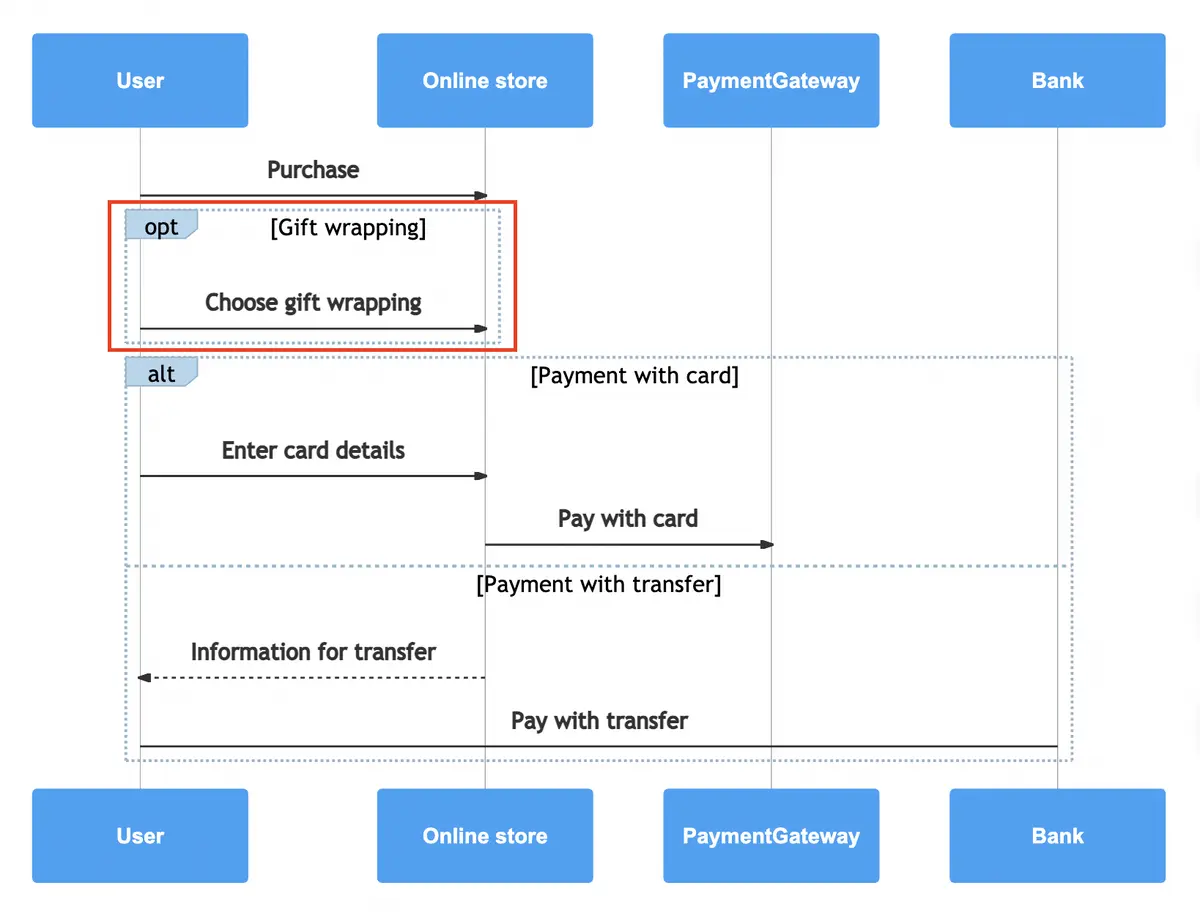
\includegraphics[width=0.75\textwidth]{combined-fragment.png}
\end{figure}

\clearpage

\section{Design Pattern}
\begin{center}
    \textit{``I Design Pattern sono descrizioni di classi e oggetti comunicanti, personalizzate per
risolvere un problema di progettazione generale all'interno di un contesto particolare.''}
\end{center}

\noindent Elementi cardine:
\begin{enumerate}
    \item \textbf{Name}
    \item \textbf{Problem}
    \item \textbf{Solution}
    \item \textbf{Consequences}
\end{enumerate}

\noindent Vengono divisi in Pattern:
\begin{itemize}
    \item \textbf{Creazionali}: istanziazione di oggetti
    \item \textbf{Strutturali}: composizione di classi e oggetti per realizzare strutture logiche più ampie e flessibili
    \item \textbf{Comportamentali}: interazioni tra oggetti, assegnazione delle responsabilità e flussi di controllo dinamici
\end{itemize}

\newpage

\subsection{Pattern Creazionali}

\paragraph{Singleton Pattern} \underline{Garantisce che una classe possieda un'unica istanza accessibile globalmente}:
\begin{lstlisting}[language=Java]
class Singleton {
    // Unica istanza statica (app. alla classe stessa, non all'oggetto)
    private static Singleton theIstance = null;

    // Costruttore privato
    private Singleton() {}

    // Metodo statico pubblico (unica porta d'ingresso)
    public static Singleton getIstance() {
        if (theIstance == null) theIstance = new Singleton();
        return theIstance;
    }
}
\end{lstlisting}

\noindent Il costruttore privato vieta il comando \texttt{new}, solo la classe stessa può chiamare il costruttore

\begin{figure}[htbp]
\centering
\begin{tikzpicture}[
    font=\small\sffamily,
    cls/.style={draw, semithick, rectangle split, rectangle split parts=3, fill=blue!6, text width=5.2cm, align=left, inner sep=5pt},
    note/.style={draw, semithick, fill=yellow!20, font=\scriptsize\ttfamily, inner sep=4pt}
]
    \node[cls] (s) at (0, 0) {
        \cn{Singleton}
        \nodepart{second}
        \texttt{- static uniqueInstance : Singleton}\\
        \texttt{- singletonData}
        \nodepart{third}
        \texttt{+ static instance() : Singleton}\\
        \texttt{+ SingletonOperation()}\\
        \texttt{+ GetSingletonData()}
    };
    \node[note, right=1.6cm of s] (n) {return uniqueInstance;};
    \draw[dashed, semithick] (s.three east) -- (n.west);
\end{tikzpicture}
\caption{Diagramma delle classi del pattern Singleton con metodo di accesso statico.}
\label{fig:pattern_singleton_structure}
\end{figure}

\newpage

\paragraph{Builder Pattern} \underline{Separa la costruzione di un oggetto complesso dalla sua rappresentazione}. L'unità \texttt{Director} viene delegata del compito di costruzione, ma demanda la realizzazione fisica dei singoli componenti ad un'interfaccia astratta \texttt{Builder}, mentre i \texttt{ConcreteBuilder} realizzano le parti specifiche.

\begin{figure}[htbp]
\centering
\begin{tikzpicture}[
    font=\footnotesize\sffamily,
    cls/.style={draw, semithick, rectangle split, rectangle split parts=2, fill=blue!5, text width=3.4cm, align=left, inner sep=4pt},
    inh/.style={-{Triangle[open, length=7pt, width=6pt]}, semithick},
    assoc/.style={semithick, -{Stealth[scale=0.9]}},
    note/.style={draw, semithick, fill=yellow!20, font=\scriptsize\sffamily, text width=3.2cm, inner sep=3pt}
]
    \node[cls, text width=2.4cm] (dir) at (-4.2, 2.4) {\cn{Director}\nodepart{second}+build()};
    \node[cls, text width=3.2cm, fill=orange!8] (bld) at (1.8, 2.4) {\cn{\textit{Builder}}\nodepart{second}+buildPart()};
    \draw[assoc] (dir.east) -- node[above, font=\scriptsize\sffamily] {uses / assembles} (bld.west);

    \node[cls, text width=3.2cm] (b1) at (-0.4, -0.6) {\cn{ComponentBuilder 1}\nodepart{second}+buildPart()};
    \node[cls, text width=3.2cm] (bn) at (4.0, -0.6) {\cn{ComponentBuilder n}\nodepart{second}+buildPart()};

    \coordinate (fork) at (1.8, 1.2);
    \draw[inh] (fork) -- (bld.south);
    \draw[semithick] (b1.north) -- (b1.north |- fork) -- (bn.north |- fork) -- (bn.north);

    \node[cls, text width=2.8cm, fill=green!8] (prod) at (-4.2, -0.6) {\cn{Product}\nodepart{second}Component 1\\ \dots\\ Component n};
    \draw[assoc, dashed] (b1.west) -- node[above, font=\scriptsize\sffamily] {builds} (prod.east);

    \node[note] (n) at (-4.2, 4.4) {Per ogni componente:\\ invoca il builder appropriato};
    \draw[dashed, semithick] (dir.north) -- (n.south);
\end{tikzpicture}
\caption{Diagramma di classe formale del pattern Builder.}
\label{fig:pattern_builder_structure}
\end{figure}

\noindent È utile l'analogia della costruzione di una \underline{casa} (\textit{Oggetto complesso}). L'\underline{architetto} è il \textit{Builder}, conosce l'ordine di esecuzione e creazione ma non l'implementazione effettiva. Quest'ultima viene delegata dall'architetto all'\underline{ingegnere} (\textit{Builder}) che ha i metodi per iniziare l'implementazione effettiva. La realizzazione concreta viene a sua volta delegata ai \underline{muratori} (\textit{ComponentBuilder}).

\newpage

\paragraph{Abstract Factory Pattern} \underline{Fornire un'interfaccia per creare famiglie di oggetti correlati o} \\\underline{dipendenti tra loro senza specificare le loro classi concrete}.

\begin{figure}[htbp]
\centering
\begin{tikzpicture}[
    font=\scriptsize\sffamily,
    cls/.style={draw, semithick, rectangle split, rectangle split parts=2, fill=blue!5, text width=3.6cm, align=left, inner sep=3pt},
    inh/.style={-{Triangle[open, length=6pt, width=5pt]}, semithick}
]
    % Fabbriche
    \node[cls, fill=orange!8] (af) at (-4.2, 3.2) {\cn{\textit{AbstractFactory}}\nodepart{second}+createComponent1()\\ \dots\\ +createComponentN()};
    \node[cls, text width=3.0cm] (fa) at (-6.0, 0.4) {\cn{FamilyAFactory}\nodepart{second}+createComponent1()\\ \dots};
    \node[cls, text width=3.0cm] (fz) at (-2.4, 0.4) {\cn{FamilyZFactory}\nodepart{second}+createComponent1()\\ \dots};
    \draw[inh] (fa.north) -- ++(0, 0.4) -| (af.south);
    \draw[inh] (fz.north) -- ++(0, 0.4) -| (af.south);

    % Componenti Prodotto
    \node[cls, fill=orange!8, text width=3.2cm] (ac1) at (3.6, 3.2) {\cn{\textit{AbstractComponent 1}}\nodepart{second}\dots};
    \node[cls, text width=2.8cm] (c1a) at (1.8, 0.4) {\cn{FamilyAComponent 1}\nodepart{second}\dots};
    \node[cls, text width=2.8cm] (c1z) at (5.4, 0.4) {\cn{FamilyZComponent 1}\nodepart{second}\dots};
    \draw[inh] (c1a.north) -- ++(0, 0.4) -| (ac1.south);
    \draw[inh] (c1z.north) -- ++(0, 0.4) -| (ac1.south);
\end{tikzpicture}
\caption{Architettura a famiglie e componenti del pattern Abstract Factory.}
\label{fig:pattern_abstract_factory}
\end{figure}

\noindent Analogia: UI per diversi SO (Mac, Windows). Non voglio fare ogni volta \texttt{if (Mac) ... else ...}

\begin{lstlisting}[language=Java]
// Configurazione del client con una specifica famiglia:
AbstractFactory f;
AbstractComponent1 c1;
AbstractComponent2 c2;

// Prelievo del componente 1 appartenente alla Famiglia A:
f = new FamilyAFactory();
c1 = f.createComponent1();

// Passaggio trasparente alla Famiglia C:
f = new FamilyCFactory();
c2 = f.createComponent2();
\end{lstlisting}

\noindent Uso una \textit{Super-Fabbrica}. I ruoli sono:
\begin{itemize}
    \item \textbf{AbstractFactory}: interface che chiama \texttt{Button createButton()}, metodo di creazione per tutti i tipi di famiglia (Mac e Windows usano sempre \texttt{createButton()})
    \item \textbf{ConcreteFactory}: una per famiglia, \texttt{WindowsFactory}
    \item \textbf{AbstractProduct}: interfaccia per prodotto (\texttt{Button})
    \item \textbf{ConcreteProduct}: una per famiglia (\texttt{WindowsButton})
\end{itemize}

\newpage

\paragraph{Factory Method Pattern} \underline{Definisce un'interfaccia per creare un oggetto, lasciando che siano le} \\underline{sottoclassi a decidere quale classe concreta istanziare}.

\begin{figure}[htbp]
\centering
\begin{tikzpicture}[
    font=\footnotesize\sffamily,
    cls/.style={draw, semithick, rectangle split, rectangle split parts=2, fill=blue!5, text width=3.4cm, align=left, inner sep=4pt},
    inh/.style={-{Triangle[open, length=7pt, width=6pt]}, semithick},
    assoc/.style={semithick, -{Stealth[scale=0.9]}, dashed}
]
    % Prodotti
    \node[cls, fill=orange!8] (prod) at (4.0, 2.6) {\cn{\textit{Product}}\nodepart{second}\dots};
    \node[cls] (cprod) at (4.0, -0.4) {\cn{ConcreteProduct}\nodepart{second}\dots};
    \draw[inh] (cprod.north) -- (prod.south);

    % Creatori
    \node[cls, fill=orange!8] (cr) at (-3.4, 2.6) {\cn{\textit{AbstractCreator}}\nodepart{second}+\textit{FactoryMethod()} : Product};
    \node[cls] (cc1) at (-3.4, -0.4) {\cn{ConcreteCreator 1}\nodepart{second}+FactoryMethod() : Product};
    \draw[inh] (cc1.north) -- (cr.south);

    % Dipendenza di creazione
    \draw[assoc] (cc1.east) -- node[above, font=\scriptsize\sffamily] {istanzia} (cprod.west);
\end{tikzpicture}
\caption{Factory Method: delega dell'istanziazione alle sottoclassi.}
\label{fig:pattern_factory_method}
\end{figure}

\noindent Immaginiamo un'azienda di trasporti. Non sa a priori se il trasporto avverrà via terra (truck) o via mare (ship), quindi la classe Logistics usa un factory method che sarà sovrascritto tramite method overriding dalle sottoclassi:

\begin{lstlisting}[language=Java]
// 1. Product: interfaccia comune
interface Transport { ... }

// 2. ConcreteProducts: le implementazioni specifiche
class Truck implements Transport { ... }

class Ship implements Transport { ... }

// 3. Creator: contiene la logica di business, ma delega la creazione!
abstract class Logistics {
    
    // Factory Method
    public abstract Transport createTransport();

    // Lavora con Transport senza sapere se e' Truck o Ship
    public void planDelivery() {
        Transport t = createTransport(); // Chiama il factory method!
        t.deliver();
    }
}

// 4. ConcreteCreators: decidono quale oggetto creare
class RoadLogistics extends Logistics {
    @Override
    public Transport createTransport() {
        return new Truck(); // Istanzia il prodotto concreto
    }
}

class SeaLogistics extends Logistics {
    @Override
    public Transport createTransport() {
        return new Ship(); // Istanzia l'altro prodotto concreto
    }
}

// Utilizzo
public class Main {
    public static void main(String[] args) {
        Logistics logisticaTerrestre = new RoadLogistics();
        logisticaTerrestre.planDelivery(); // Output: Consegna via terra in camion.

        Logistics logisticaMarittima = new SeaLogistics();
        logisticaMarittima.planDelivery(); // Output: Consegna via mare in nave.
    }
}
\end{lstlisting}

\newpage

\paragraph{Prototype Pattern} \underline{Specifica gli oggetti da creare usando un prototipo e crea i nuovi oggetti}\\\underline{clonando tale prototipo}.

\begin{figure}[htbp]
\centering
\begin{tikzpicture}[
    font=\footnotesize\sffamily,
    cls/.style={draw, semithick, rectangle split, rectangle split parts=2, fill=blue!5, text width=3.4cm, align=left, inner sep=4pt},
    inh/.style={-{Triangle[open, length=7pt, width=6pt]}, semithick},
    assoc/.style={semithick, -{Stealth[scale=0.9]}}
]
    \node[cls, text width=2.4cm] (cl) at (-4.2, 2.4) {\cn{Client}\nodepart{second}+operation()};
    \node[cls, text width=3.2cm, fill=orange!8] (proto) at (2.0, 2.4) {\cn{\textit{Prototype}}\nodepart{second}+\textit{Clone()} : Prototype};
    \draw[assoc] (cl.east) -- node[above, font=\scriptsize\sffamily] {p = proto.Clone()} (proto.west);

    \node[cls, text width=3.2cm] (p1) at (-0.2, -0.6) {\cn{ConcretePrototype 1}\nodepart{second}+Clone() : Prototype};
    \node[cls, text width=3.2cm] (pn) at (4.2, -0.6) {\cn{ConcretePrototype n}\nodepart{second}+Clone() : Prototype};

    \coordinate (fork) at (2.0, 1.2);
    \draw[inh] (fork) -- (proto.south);
    \draw[semithick] (p1.north) -- (p1.north |- fork) -- (pn.north |- fork) -- (pn.north);
\end{tikzpicture}
\caption{Diagramma delle classi del pattern Prototype con metodo \texttt{Clone()}.}
\label{fig:pattern_prototype}
\end{figure}

\begin{lstlisting}[language=Java]
// 1. Prototype: interfaccia comune con il metodo clone
interface Shape {
    Shape clone();
    void draw();
}

// 2. ConcretePrototype: implementa la clonazione copiando i propri campi
class Circle implements Shape {
    ...
    @Override
    public Shape clone() {
        // Restituisce un nuovo oggetto identico all'originale
        return new Circle(this);
    }

    @Override
    public void draw() {
        System.out.println("Cerchio ...")
    }
}

public class Main {
    public static void main(String[] args) {
        // Creo e configuro il prototipo UNA sola volta
        Shape prototipoCerchioRosso = new Circle(50, "Rosso");

        // Clono quando serve
        Shape copia1 = prototipoCerchioRosso.clone();
        Shape copia2 = prototipoCerchioRosso.clone();

        copia1.draw(); // Output: Cerchio [raggio=50, colore=Rosso]
        copia2.draw(); // Output: Cerchio [raggio=50, colore=Rosso]
    }
}
\end{lstlisting}

\newpage
\subsection{Pattern Strutturali}
\paragraph{Composite Pattern} \underline{Compone gli oggetti in strutture ad albero, permettendo al client di trattare }\\\underline{ugualmente foglie e nodi compositi}.

\begin{figure}[htbp]
\centering
\begin{tikzpicture}[
    font=\footnotesize\sffamily,
    cls/.style={draw, semithick, rectangle split, rectangle split parts=2, fill=blue!5, text width=3.3cm, align=left, inner sep=4pt},
    cls3/.style={draw, semithick, rectangle split, rectangle split parts=3, fill=blue!5, text width=3.3cm, align=left, inner sep=4pt},
    inh/.style={-{Triangle[open, length=7pt, width=6pt]}, semithick},
    aggr/.style={{Diamond[open, length=8pt, width=5pt]}-, semithick},
    note/.style={draw, semithick, fill=yellow!20, font=\scriptsize\ttfamily, text width=3.2cm, inner sep=3pt}
]
    \node[cls, text width=2.4cm] (b) at (-4.2, 3) {\cn{Budget}\nodepart{second}\dots};
    \node[cls3, text width=3.6cm, fill=orange!8] (acc) at (1.8, 3) {\cn{\textit{Account}}\nodepart{second}\dots\nodepart{third}+GlobalOperation()\\ +AtomicOperation()\\ +Add(Account)\\ +Remove(Account)};
    \draw[aggr] (b.east) -- node[above, font=\scriptsize\sffamily, pos=0.88] {$*$} (acc.west);

    \node[cls3, text width=3.6cm] (sa) at (-1.8, -0.6) {\cn{SimpleAccount}\nodepart{second}\dots\nodepart{third}+GlobalOperation()\\ +AtomicOperation()\\ +Operation()};
    \node[cls3, text width=3.6cm] (ca) at (4.2, -0.6) {\cn{CompositeAccount}\nodepart{second}\dots\nodepart{third}+GlobalOperation()\\ +AtomicOperation()\\ +Add(Account)\\ +Remove(Account)};

    \coordinate (fork) at (1.8, 1.3);
    \draw[inh] (fork) -- (acc.south);
    \draw[semithick] (sa.north) -- (sa.north |- fork) -- (ca.north |- fork) -- (ca.north);

    % Aggregazione ricorsiva
    \draw[aggr] (ca.east) -- ++(1.4, 0) |- node[near end, right, font=\scriptsize\sffamily] {children $*$} (acc.east);

    % Note esplicative
    \node[note] (n1) at (5.2, -3.2) {forall g in children:\\ \quad g.GlobalOperation();};
    \draw[dashed, semithick] (ca.south) -- (n1.north);
\end{tikzpicture}
\caption{Modellazione dei conti del bilancio mediante il pattern Composite.}
\label{fig:scenario_composite_accounts}
\end{figure}

\noindent Calcolo del prezzo totale di una spedizione Amazon: ci sono prodotti singoli (foglie) e scatole (nodi compositi)

\begin{lstlisting}[language=Java]
// 1. COMPONENT: l'interfaccia comune
interface OrderItem {
    double getPrice(); // Operazione uniforme: "dimmi quanto costi"
}
// 2. LEAF (Foglia): il singolo prodotto con un suo prezzo
class Product implements OrderItem {
    private String name;
    private double price;

    public Product(String name, double price) {
        this.name = name;
        this.price = price;
    }

    @Override
    public double getPrice() {
        return this.price; // Restituisce semplicemente il proprio prezzo
    }
}

// 3. COMPOSITE (Contenitore): la scatola Amazon
class Box implements OrderItem {
    private String label;
    // La lista contiene OrderItem: quindi accetta Product e altre Box!
    private List<OrderItem> children = new ArrayList<>();

    public Box(String label) {
        this.label = label;
    }
    public void add(OrderItem item) {
        children.add(item);
    }
    public void remove(OrderItem item) {
        children.remove(item);
    }

    @Override
    public double getPrice() {
        double total = 0;
        // Delega a cascata a tutto cio' che c'e' dentro la scatola
        for (OrderItem item : children) {
            total += item.getPrice();
        }
        return total;
    }
}

// CLIENT: il sistema di checkout di Amazon
public class AmazonOrderDemo {
    public static void main(String[] args) {
        // Creo i singoli prodotti (Foglie)
        OrderItem libro = new Product("Design Patterns GoF", 40.0);
        OrderItem cuffie = new Product("Cuffie Bluetooth", 60.0);
        OrderItem cavoUsb = new Product("Cavo USB-C", 10.0);

        // Creo una scatola
        Box scatolaElettronica = new Box("Scatola Elettronica");
        scatolaElettronica.add(cuffie);
        scatolaElettronica.add(cavoUsb);
        // Creo il pacco grande finale
        Box paccoGrande = new Box("Pacco Ordine Completo");
        paccoGrande.add(libro);
        paccoGrande.add(scatolaElettronica);

        // Il sistema chiama getPrice() senza sapere se e' un singolo articolo o una matrioska di scatole!
        System.out.println("Singolo libro: " + libro.getPrice()); // 40
        System.out.println("Scatola elettronica: " + scatolaElettronica.getPrice()); // 70
        System.out.println("Totale ordine: " + paccoGrande.getPrice()); // 110
    }
}
\end{lstlisting}

\newpage

\paragraph{Adapter Pattern} \underline{Converte l'interfaccia di una classe esistente Adaptee in un'altra interfaccia}\\\underline{ Target attesa dal client, permettendo la comunicazione tra due classi incompatibili}.

\begin{figure}[htbp]
\centering
\begin{tikzpicture}[
    font=\footnotesize\sffamily,
    cls/.style={draw, semithick, rectangle split, rectangle split parts=2, fill=blue!5, text width=3.4cm, align=left, inner sep=4pt},
    inh/.style={-{Triangle[open, length=7pt, width=6pt]}, semithick},
    assoc/.style={semithick, -{Stealth[scale=0.9]}},
    note/.style={draw, semithick, fill=yellow!20, font=\scriptsize\ttfamily, inner sep=3pt}
]
    \node[cls, text width=2.4cm] (cl) at (-4.2, 2.4) {\cn{Client}\nodepart{second}\dots};
    \node[cls, text width=3.0cm, fill=orange!8] (tgt) at (0, 2.4) {\cn{\textit{Target}}\nodepart{second}+\textit{Request()}};
    \node[cls, text width=3.4cm] (adp) at (5.2, 2.4) {\cn{Adaptee}\nodepart{second}+SpecificRequest()};

    \node[cls, text width=3.0cm] (ada) at (0, -0.6) {\cn{Adapter}\nodepart{second}+Request()};

    \draw[assoc] (cl.east) -- (tgt.west);
    \draw[inh] (ada.north) -- (tgt.south);
    \draw[assoc] (ada.east) -| node[pos=0.25, above, font=\scriptsize\sffamily] {adaptee} (adp.south);

    \node[note] (n) at (0, -2.4) {adaptee->SpecificRequest();};
    \draw[dashed, semithick] (ada.south) -- (n.north);
\end{tikzpicture}
\caption{Object Adapter: disaccoppiamento mediante composizione d'oggetto e delega.}
\label{fig:pattern_adapter_object}
\end{figure}

\noindent Immaginiamo di volere una classe Target \texttt{PayPalPayment} avendo una vecchia classe Adaptee \texttt{LegacyBankAPI}. Posso fare:
\begin{lstlisting}[language=Java]
// 1. TARGET: l'interfaccia moderna che il tuo e-commerce si aspetta
interface PayPalPayment {
    void pay(double euros); // Equivale a Request()
}

// 2. ADAPTEE: la libreria esterna incompatibile (non modificabile!)
class LegacyBankAPI {
    public void executeWireTransfer(int cents) { // Equivale a SpecificRequest()
        System.out.println("Bonifico bancario eseguito di: " + cents + " centesimi.");
    }
}

// 3. ADAPTER: implementa il Target e avvolge (wrappa) l'Adaptee
class BankAdapter implements PayPalPayment {
    private LegacyBankAPI bankApi; // Riferimento all'Adaptee (composizione)

    public BankAdapter(LegacyBankAPI bankApi) {
        this.bankApi = bankApi;
    }

    @Override
    public void pay(double euros) {
        // Traduce il formato (da euro double a centesimi int) e delega
        int cents = (int) Math.round(euros * 100);
        bankApi.executeWireTransfer(cents);
    }
}

// 4. CLIENT: il checkout dell'e-commerce
public class EcommerceDemo {
    public static void main(String[] args) {
        LegacyBankAPI vecchiaBanca = new LegacyBankAPI();

        // Avvolgo la libreria incompatibile nell'Adapter
        PayPalPayment processor = new BankAdapter(vecchiaBanca);

        // Il checkout chiama il metodo standard senza accorgersi della traduzione!
        processor.pay(49.90);
        // Output: Bonifico bancario eseguito di: 4990 centesimi.
    }
}
\end{lstlisting}

\noindent Sto quindi usando un intermediario, un po' come la funzione swap che ha bisogno di temp per far ``comunicare'' i due elementi da swappare.

\newpage

\paragraph{Bridge Pattern} \underline{Disaccoppia un'astrazione dalla sua implementazione in modo che le due}\\\underline{ possano variare indipendentemente, evitando un numero esponenziale di sottoclassi}.

\begin{figure}[htbp]
\centering
\begin{tikzpicture}[
    font=\footnotesize\sffamily,
    cls/.style={draw, semithick, rectangle split, rectangle split parts=2, fill=blue!5, text width=3.4cm, align=left, inner sep=4pt},
    inh/.style={-{Triangle[open, length=7pt, width=6pt]}, semithick},
    aggr/.style={{Diamond[open, length=8pt, width=5pt]}-, semithick},
    note/.style={draw, semithick, fill=yellow!20, font=\scriptsize\ttfamily, inner sep=3pt}
]
    \node[draw, semithick, fill=white, inner sep=4pt] (cl) at (-5.2, 2.4) {Client};
    \node[cls, fill=orange!8, text width=3.0cm] (abs) at (-1.8, 2.4) {\cn{\textit{Abstraction}}\nodepart{second}+Operation()};
    \node[cls, fill=orange!8, text width=3.4cm] (imp) at (4.0, 2.4) {\cn{\textit{Implementor}}\nodepart{second}+OperationImp()};

    \node[cls, text width=3.2cm] (rabs) at (-1.8, -0.6) {\cn{RefinedAbstraction}\nodepart{second}\dots};
    \node[cls, text width=3.0cm] (cia) at (2.2, -0.6) {\cn{ConcreteImplA}\nodepart{second}+OperationImp()};
    \node[cls, text width=3.0cm] (cib) at (5.8, -0.6) {\cn{ConcreteImplB}\nodepart{second}+OperationImp()};

    \draw[-{Stealth[scale=0.9]}, semithick] (cl) -- (abs);
    \draw[aggr] (abs.east) -- node[above, font=\scriptsize\sffamily] {imp} (imp.west);
    \draw[inh] (rabs.north) -- (abs.south);

    \coordinate (fork) at (4.0, 1.2);
    \draw[inh] (fork) -- (imp.south);
    \draw[semithick] (cia.north) -- (cia.north |- fork) -- (cib.north |- fork) -- (cib.north);

    \node[note] (n) at (-1.8, 4.2) {imp->OperationImp();};
    \draw[dashed, semithick] (abs.north) -- (n.south);
\end{tikzpicture}
\caption{Diagramma delle classi del pattern Bridge: separazione tra gerarchia di astrazione e implementazione.}
\label{fig:pattern_bridge_structure}
\end{figure}

\noindent Immaginiamo l'albero d'astrazione come la classe \texttt{Telecomando} e la sua estensione \texttt{TelecomandoPro}, poi l'albero implementatore, con la classe \texttt{Dispositivo} e le sue implementazioni \texttt{TV} e \texttt{Radio}. Il client potrà combinare liberamente qualsiasi telecomando con qualsiasi dispositivo:
\begin{lstlisting}[language=Java]
public class BridgeDemo {
    public static void main(String[] args) {
        Device miaTv = new Tv();
        RemoteControl telecomandoBase = new RemoteControl(miaTv);
        telecomandoBase.powerOn(); // Output: TV accesa

        Device miaRadio = new Radio();
        AdvancedRemote telecomandoPro = new AdvancedRemote(miaRadio);
        telecomandoPro.powerOn();  // Output: Radio accesa
        telecomandoPro.mute();     // Output: Premuto tasto Muto
    }
}
\end{lstlisting}

\newpage

\paragraph{Decorator Pattern} \underline{Allega dinamicamente responsabilità aggiuntive ad un singolo oggetto a }\\\underline{runtime senza alterarne l'interfaccia}.

\begin{figure}[htbp]
\centering
\begin{tikzpicture}[
    font=\footnotesize\sffamily,
    cls/.style={draw, semithick, rectangle split, rectangle split parts=1, fill=blue!5, text width=3.2cm, align=center, inner sep=5pt},
    inh/.style={-{Triangle[open, length=7pt, width=6pt]}, semithick},
    aggr/.style={{Diamond[open, length=8pt, width=5pt]}-, semithick}
]
    \node[cls, fill=orange!8] (cmp) at (0, 3.2) {\guillemotleft abstract\guillemotright\\ \cn{Component}};
    \node[cls] (ccmp) at (-3.2, 1.2) {\cn{ConcreteComponent}};
    \node[cls, fill=orange!8] (dec) at (3.2, 1.2) {\cn{Decorator}};

    \draw[inh] (ccmp.north) -- ++(0, 0.6) -| (cmp.south);
    \draw[inh] (dec.north) -- ++(0, 0.6) -| (cmp.south);

    % Aggregazione Decorator -> Component
    \draw[aggr] (dec.east) -- ++(1.4, 0) |- (cmp.east);

    \node[cls] (cd1) at (1.4, -1.0) {\cn{ConcreteDecorator 1}};
    \node[cls] (cdn) at (5.0, -1.0) {\cn{ConcreteDecorator n}};

    \coordinate (fork) at (3.2, 0.2);
    \draw[inh] (fork) -- (dec.south);
    \draw[semithick] (cd1.north) -- (cd1.north |- fork) -- (cdn.north |- fork) -- (cdn.north);
\end{tikzpicture}
\caption{Diagramma strutturale del pattern Decorator.}
\label{fig:pattern_decorator_structure}
\end{figure}

\noindent Immaginiamo di avere una persona che indossa solamente una \texttt{Maglietta} e in base alla situazione aggiungiamo \texttt{Maglione}, \texttt{Impermeabile}, ...:

\begin{lstlisting}[language=Java]
// 1. COMPONENT: l'interfaccia comune a tutti i capi/strati
interface Outfit {
    String getDescription(); // Descrive cosa indossi
    int getWarmthLevel();    // Calcola il livello di calore totale
}

// 2. CONCRETE COMPONENT: lo strato base indispensabile (la maglietta)
class TShirt implements Outfit {
    @Override
    public String getDescription() {
        return "Maglietta di cotone";
    }

    @Override
    public int getWarmthLevel() {
        return 1; // Calore base = 1
    }
}

// 3. DECORATOR: il "guscio" astratto che avvolge UN solo altro capo
abstract class ClothingDecorator implements Outfit {
    protected Outfit wrappedOutfit; // Ref. (1) allo strato sottostante

    public ClothingDecorator(Outfit outfit) {
        this.wrappedOutfit = outfit;
    }

    @Override
    public String getDescription() {
        return wrappedOutfit.getDescription();
    }

    @Override
    public int getWarmthLevel() {
        return wrappedOutfit.getWarmthLevel();
    }
}

// 4. CONCRETE DECORATORS: i singoli indumenti aggiuntivi
class SweaterDecorator extends ClothingDecorator {
    public SweaterDecorator(Outfit outfit) {
        super(outfit);
    }

    @Override
    public String getDescription() {
        // Prende cio' che c'e' sotto + aggiunge se' stesso
        return super.getDescription() + " + Maglione di lana";
    }

    @Override
    public int getWarmthLevel() {
        // Prende il calore sottostante + aggiunge 4 punti calore
        return super.getWarmthLevel() + 4;
    }
}

class RaincoatDecorator extends ClothingDecorator {
    public RaincoatDecorator(Outfit outfit) {
        super(outfit);
    }

    @Override
    public String getDescription() {
        return super.getDescription() + " + Impermeabile antivento";
    }

    @Override
    public int getWarmthLevel() {
        return super.getWarmthLevel() + 2;
    }
}

// CLIENT: si veste dinamico in base al meteo!
public class WinterOutfitDemo {
    public static void main(String[] args) {
        // Mattina in casa: solo maglietta (ConcreteComponent)
        Outfit mioOutfit = new TShirt();
        System.out.println("In casa: " + mioOutfit.getDescription() + " | Calore: " + mioOutfit.getWarmthLevel());
        // Output: In casa: Maglietta di cotone | Calore: 1

        // Esce e fa freddo: "decora" la maglietta con il maglione
        mioOutfit = new SweaterDecorator(mioOutfit);
        System.out.println("Fuori col freddo: " + mioOutfit.getDescription() + " | Calore: " + mioOutfit.getWarmthLevel());
        // Output: Fuori col freddo: Maglietta di cotone + Maglione di lana | Calore: 5

        // Inizia anche a piovere: "decora" tutto con l'impermeabile
        mioOutfit = new RaincoatDecorator(mioOutfit);
        System.out.println("Con la pioggia: " + mioOutfit.getDescription() + " | Calore: " + mioOutfit.getWarmthLevel());
        // Output: Con la pioggia: Maglietta di cotone + Maglione di lana + Impermeabile antivento | Calore: 7
    }
}
\end{lstlisting}

\paragraph{Proxy Pattern} \underline{Fornisce un placeholder per controllare l'accesso ad un oggetto reale, esponendo la }\\\underline{stessa interfaccia}.

\begin{figure}[htbp]
\centering
\begin{tikzpicture}[
    font=\footnotesize\sffamily,
    cls/.style={draw, semithick, rectangle split, rectangle split parts=2, fill=blue!5, text width=3.2cm, align=left, inner sep=4pt},
    inh/.style={-{Triangle[open, length=7pt, width=6pt]}, semithick},
    assoc/.style={semithick, -{Stealth[scale=0.9]}},
    note/.style={draw, semithick, fill=yellow!20, font=\scriptsize\ttfamily, inner sep=3pt}
]
    % Client e Interfaccia Subject
    \node[cls, text width=2.2cm] (cl) at (-4.6, 2.6) {\cn{Client}\nodepart{second}\dots};
    \node[cls, fill=orange!8, text width=3.2cm] (subj) at (0, 2.6) {\cn{\textit{Subject}}\nodepart{second}+\textit{Request()}};

    % Sottoclassi RealEntity e Proxy
    \node[cls, text width=3.2cm] (real) at (-2.4, -0.4) {\cn{RealEntity}\nodepart{second}+Request()};
    \node[cls, text width=3.2cm] (prx) at (2.4, -0.4) {\cn{Proxy}\nodepart{second}+Request()};

    % Relazioni di associazione ed ereditarietà
    \draw[assoc] (cl.east) -- (subj.west);

    \coordinate (fork) at (0, 1.3);
    \draw[inh] (fork) -- (subj.south);
    \draw[semithick] (real.north) -- (real.north |- fork) -- (prx.north |- fork) -- (prx.north);

    % Riferimento dal Proxy al RealEntity
    \draw[assoc] (prx.west) -- node[above, font=\scriptsize\sffamily] {realEntity} (real.east);

    % Nota esplicita sulla delega
    \node[note] (n) at (2.4, -2.2) {realEntity->Request();};
    \draw[dashed, semithick] (prx.south) -- (n.north);
\end{tikzpicture}
\caption{Diagramma delle classi del pattern Proxy con delega controllata a \texttt{RealEntity}.}
\label{fig:pattern_proxy_structure}
\end{figure}

\noindent Immaginiamo un'oggetto reale come i contanti e il proxy come la carta di credito, che funge da placeholder per l'oggetto reale (contanti) facendo prima dei controlli.

\newpage
\subsection{Pattern Comportamentali}
\paragraph{Iterator Pattern} \underline{Fornisce un modo per accedere sequenzialmente agli elementi di un oggetto}\\\underline{aggregato senza esporne la rappresentazione interna}.

\begin{figure}[htbp]
\centering
\begin{tikzpicture}[
    font=\footnotesize\sffamily,
    cls/.style={draw, semithick, rectangle split, rectangle split parts=2, fill=blue!5, text width=3.2cm, align=left, inner sep=4pt},
    inh/.style={-{Triangle[open, length=7pt, width=6pt]}, semithick},
    assoc/.style={semithick, -{Stealth[scale=0.9]}}
]
    \node[cls, text width=3.2cm] (list) at (-3.8, 2.4) {\cn{ListOfAccounts}\nodepart{second}+CreateIterator()};
    \node[cls, text width=2.4cm, fill=green!8] (b) at (0.2, 3.8) {\cn{Budget}};
    \node[cls, text width=3.0cm, fill=orange!8] (it) at (4.0, 2.4) {\cn{\textit{Iterator}}\nodepart{second}+First()\\ +Next()\\ +IsDone()\\ +CurrentItem()};
    \node[cls, text width=3.0cm] (ait) at (4.0, -0.6) {\cn{AccountsIterator}\nodepart{second}\dots};

    \draw[assoc] (b) -- (list);
    \draw[assoc] (b) -- (it);
    \draw[inh] (ait.north) -- (it.south);
    \draw[assoc] (list.south) -- ++(0, -0.6) -| node[near start, below, font=\scriptsize\sffamily] {crea istanza} (ait.west);
    \draw[assoc, dashed] (ait.north west) -- node[above, sloped, font=\scriptsize\sffamily] {riferimento a} (list.south east);
\end{tikzpicture}
\caption{Disaccoppiamento della scansione dei conti mediante il pattern Iterator.}
\label{fig:scenario_iterator_accounts}
\end{figure}

\noindent Immaginiamo una collezione di oggetti (\texttt{ListOfAccounts}). Vogliamo permettere al client (\texttt{Budget}) di scorrere tutti gli elementi sequenzialmente evitando l'esposizione alla struttura interna e sovraccarico di responsabilità.

\paragraph{Visitor Pattern} \underline{Rappresenta un'operazione da eseguire sugli elementi di una struttura di }\\\underline{oggetti, consentendo di definire nuove operazioni senza modificare le classi degli elementi}. 

\begin{figure}[htbp]
\centering
\begin{tikzpicture}[
    font=\footnotesize\sffamily,
    cls/.style={draw, semithick, rectangle split, rectangle split parts=2, fill=blue!5, text width=2.8cm, align=left, inner sep=4pt},
    inh/.style={-{Triangle[open, length=6pt, width=5pt]}, semithick},
    assoc/.style={semithick, -{Stealth[scale=0.85]}, dashed},
    note/.style={draw, semithick, fill=yellow!20, font=\scriptsize\ttfamily, text width=2.8cm, inner sep=3pt}
]
    % Struttura Elementi
    \node[cls, fill=orange!8, text width=3.4cm] (elem) at (0, 3.4) {\cn{\textit{Element}}\nodepart{second}+\textit{accept(Visitor v)}};
    \node[cls, text width=2.4cm] (l1) at (-3.4, 1.4) {\cn{Leaf 1}\nodepart{second}+accept(v)};
    \node[cls, text width=2.4cm] (l2) at (0, 1.4) {\cn{Leaf 2}\nodepart{second}+accept(v)};
    \node[cls, text width=2.6cm] (comp) at (3.4, 1.4) {\cn{Composite}\nodepart{second}+accept(v)};

    \coordinate (efork) at (0, 2.5);
    \draw[inh] (efork) -- (elem.south);
    \draw[semithick] (l1.north) -- (l1.north |- efork) -- (comp.north |- efork) -- (comp.north);
    \draw[semithick] (l2.north) -- (efork);

    % Note di accettazione
    \node[note] (nl1) at (-3.4, -0.6) {v.visitX(this);};
    \draw[dashed, semithick] (l1.south) -- (nl1.north);

    % Struttura Visitor
    \node[cls, fill=red!10, text width=2.8cm] (vis) at (0, -1.6) {\cn{\textit{Visitor}}\nodepart{second}+\textit{visitX()}\\ +\textit{visitY()}};
    \node[cls, fill=red!10, text width=2.6cm] (v1) at (-1.8, -3.8) {\cn{Visitor 1}\nodepart{second}+visitX()\\ +visitY()};
    \node[cls, fill=red!10, text width=2.6cm] (vn) at (1.8, -3.8) {\cn{Visitor n}\nodepart{second}+visitX()\\ +visitY()};

    \coordinate (vfork) at (0, -2.8);
    \draw[inh] (vfork) -- (vis.south);
    \draw[semithick] (v1.north) -- (v1.north |- vfork) -- (vn.north |- vfork) -- (vn.north);

    \draw[assoc] (l1.south) -- (vis.north west);
    \draw[assoc] (comp.south) -- (vis.north east);
\end{tikzpicture}
\caption{Diagramma del pattern Visitor: separazione degli algoritmi di visita dalla struttura ad albero.}
\label{fig:pattern_visitor_structure}
\end{figure}

\noindent Gli elementi espongono \texttt{accept(Visitor v)} e tramite \textbf{Double Dispatching} invocano il metodo specifico del visitatore (\texttt{v.visitX(this)}). Nota sul double dispatching:
\begin{itemize}
    \item Primo salto: il client chiama \texttt{element.accept(visitor)}. Java risolve dinamicamente il tipo di \texttt{element}
    \item Secondo salto: dentro \texttt{Leaf1.accept(v)}, l'elemento chiama \texttt{v.visitorLeaf1(this)}. Java risolve dinamicamente il tipo di \texttt{visitor}
\end{itemize}

\paragraph{Strategy Pattern} \underline{Definisce una famiglia di algoritmi e incapsula ciascuno di essi dentro una}\\\underline{classe separata, rendendoli intercambiabili a runtime}.

\begin{figure}[htbp]
\centering
\begin{tikzpicture}[
    font=\footnotesize\sffamily,
    cls/.style={draw, semithick, rectangle split, rectangle split parts=2, fill=blue!5, text width=3.2cm, align=left, inner sep=4pt},
    inh/.style={-{Triangle[open, length=7pt, width=6pt]}, semithick},
    aggr/.style={{Diamond[open, length=8pt, width=5pt]}-, semithick},
    note/.style={draw, semithick, fill=yellow!20, font=\scriptsize\ttfamily, inner sep=3pt}
]
    \node[cls, text width=2.6cm] (ent) at (-4.0, 2.4) {\cn{Entity}\nodepart{second}+f()};
    \node[cls, fill=orange!8, text width=3.2cm] (strat) at (1.8, 2.4) {\cn{\guillemotleft abstract\guillemotright\ Strategy}\nodepart{second}+\textit{action()}};

    \draw[aggr] (ent.east) -- node[above, font=\scriptsize\sffamily] {strategy} (strat.west);

    \node[cls, text width=2.8cm] (s1) at (-0.2, -0.4) {\cn{Strategy 1}\nodepart{second}+action()};
    \node[cls, text width=2.8cm] (sn) at (3.8, -0.4) {\cn{Strategy n}\nodepart{second}+action()};

    \coordinate (fork) at (1.8, 1.2);
    \draw[inh] (fork) -- (strat.south);
    \draw[semithick] (s1.north) -- (s1.north |- fork) -- (sn.north |- fork) -- (sn.north);

    \node[note] (n) at (-4.0, 0.4) {strategy.action();};
    \draw[dashed, semithick] (ent.south) -- (n.north);
\end{tikzpicture}
\caption{Diagramma del pattern Strategy: incapsulamento ed intercambiabilità degli algoritmi.}
\label{fig:pattern_strategy_structure}
\end{figure}

\noindent Supponiamo di progettare un navigatore. Mettere tutti gli algoritmi dentro la classe principale diventerebbe enorme e illeggibile. Lo Strategy estrae ogni algoritmo dalla classe principale e lo mette in una classe separata con un'interfaccia comune:

\begin{lstlisting}[language=Java]
// 1. STRATEGY: interfaccia comune per tutti gli algoritmi di percorso
interface RouteStrategy {
    void buildRoute(String origin, String destination); // Equivale ad action()
}

// 2. CONCRETE STRATEGIES: i singoli algoritmi incapsulati in classi separate
class CarStrategy implements RouteStrategy {
    @Override
    public void buildRoute(String origin, String destination) {
        System.out.println("Percorso in AUTO da " + origin + " a " + destination + " (via autostrada, 25 min).");
    }
}

class WalkingStrategy implements RouteStrategy {
    @Override
    public void buildRoute(String origin, String destination) {
        System.out.println("Percorso A PIEDI da " + origin + " a " + destination + " (attraverso il parco, 1h 40m).");
    }
}

class BikeStrategy implements RouteStrategy {
    @Override
    public void buildRoute(String origin, String destination) {
        System.out.println("Percorso IN BICI da " + origin + " a " + destination + " (pista ciclabile, 45 min).");
    }
}

// 3. CONTEXT (Entity): il navigatore, completamente ignaro dei dettagli degli algoritmi
class Navigator {
    private RouteStrategy strategy; // Aggregazione verso Strategy

    public void setStrategy(RouteStrategy strategy) {
        this.strategy = strategy;
    }

    // Equivale a f() nel tuo diagramma
    public void navigate(String from, String to) {
        if (strategy == null) {
            System.out.println("Seleziona prima un mezzo di trasporto!");
            return;
        }
        strategy.buildRoute(from, to); // Delega pura: strategy.action();
    }
}

// CLIENT: cambia strategia dinamicamente a runtime!
public class StrategyDemo {
    public static void main(String[] args) {
        Navigator maps = new Navigator();

        // L'utente sceglie l'auto
        maps.setStrategy(new CarStrategy());
        maps.navigate("Stazione Centrale", "Universita'");

        // C'e' traffico! A runtime cambia al volo strategia senza ricreare il Navigator
        maps.setStrategy(new BikeStrategy());
        maps.navigate("Stazione Centrale", "Universita'");

        // Ha bucato la ruota: passa a piedi
        maps.setStrategy(new WalkingStrategy());
        maps.navigate("Stazione Centrale", "Universita'");
    }
}
\end{lstlisting}

\newpage
\paragraph{Chain of Responsability Pattern} \underline{Disaccoppia il mittente di una richiesta dai suoi potenziali }\\\underline{destinatari, dando a più oggetti la possibilità di gestirla lungo una catena}.

\begin{figure}[htbp]
\centering
\begin{tikzpicture}[
    font=\footnotesize\sffamily,
    cls/.style={draw, semithick, rectangle split, rectangle split parts=2, fill=blue!5, text width=3.4cm, align=left, inner sep=4pt},
    inh/.style={-{Triangle[open, length=7pt, width=6pt]}, semithick},
    assoc/.style={semithick, -{Stealth[scale=0.9]}}
]
    \node[cls, text width=2.4cm] (cl) at (-4.5, 2.4) {\cn{Client}\nodepart{second}+request()};
    \node[cls, fill=orange!8, text width=3.6cm] (h) at (1.2, 2.4) {\cn{\guillemotleft abstract\guillemotright\ Handler}\nodepart{second}-successor : Handler\\ +\textit{handleRequest(r)}};

    \draw[assoc] (cl.east) -- node[above, font=\scriptsize\sffamily] {myHandler} (h.west);
    \draw[assoc] (h.east) -- ++(1.0, 0) -- ++(0, 1.0) -| node[pos=0.25, above, font=\scriptsize\sffamily] {successor} (h.north);

    \node[cls, text width=3.2cm] (h1) at (-1.0, -0.6) {\cn{Handler 1}\nodepart{second}+handleRequest(r)};
    \node[cls, text width=3.2cm] (hn) at (3.4, -0.6) {\cn{Handler n}\nodepart{second}+handleRequest(r)};

    \coordinate (fork) at (1.2, 1.2);
    \draw[inh] (fork) -- (h.south);
    \draw[semithick] (h1.north) -- (h1.north |- fork) -- (hn.north |- fork) -- (hn.north);
\end{tikzpicture}
\caption{Diagramma del pattern Chain of Responsibility con catena ricorsiva di successori.}
\label{fig:pattern_cor_structure}
\end{figure}

\noindent Immaginiamo di avere una richiesta (ad esempio HTTP). Se il mittente (\texttt{Client}) deve sapere esattamente chi gestirà la richiesta, è costretto a mantenere riferimenti a tutti i possibili destinatari e a scrivere una lunga catena di \texttt{if-then-else}. La CoR Pattern trasforma i singoli gestori in oggetti autonomi collegati in fila come gli anelli di una catena. Ciascun anello conosce solo il proprio successore (\texttt{successor}). Quando arriva una richiesta:
\begin{itemize}
    \item L'anello valuta se è in grado di gestirla: se sì, la risolve e (di solito) ferma la catena.
    \item Se non è di sua competenza, la inoltra al successore.
\end{itemize}

\paragraph{Mediator Pattern} \underline{Definisce un oggetto che incapsula il modo in cui un insieme di }\\\underline{oggetti interagisce, evitando che si referenzino esplicitamente a vicenda (spaghetti code).}

\begin{figure}[htbp]
\centering
\begin{tikzpicture}[
    font=\footnotesize\sffamily,
    cls/.style={draw, semithick, rectangle split, rectangle split parts=2, fill=blue!5, text width=3.0cm, align=left, inner sep=4pt},
    obj/.style={draw, semithick, fill=yellow!12, text width=1.6cm, align=center, inner sep=4pt},
    inh/.style={-{Triangle[open, length=7pt, width=6pt]}, semithick},
    assoc/.style={semithick, <->, >=Stealth}
]
    \node[cls, fill=orange!8, text width=3.4cm] (med) at (0, 2.6) {\cn{\guillemotleft abstract\guillemotright\ Mediator}\nodepart{second}+f()\\ +y()\\ +z()};
    \node[cls, text width=2.8cm] (m1) at (-2.4, 0.4) {\cn{Mediator 1}\nodepart{second}\dots};
    \node[cls, text width=2.8cm] (mn) at (2.4, 0.4) {\cn{Mediator N}\nodepart{second}\dots};

    \coordinate (fork) at (0, 1.6);
    \draw[inh] (fork) -- (med.south);
    \draw[semithick] (m1.north) -- (m1.north |- fork) -- (mn.north |- fork) -- (mn.north);

    % Oggetti Colleghi Satelliti
    \node[obj] (o1) at (-4.6, 2.6) {OBJ 1};
    \node[obj] (o2) at (0, 4.6) {OBJ 2};
    \node[obj] (o3) at (4.6, 2.6) {OBJ 3};

    \draw[assoc] (o1) -- (med);
    \draw[assoc] (o2) -- (med);
    \draw[assoc] (o3) -- (med);
\end{tikzpicture}
\caption{Diagramma del pattern Mediator: accentramento delle relazioni tra colleghi.}
\label{fig:pattern_mediator_structure}
\end{figure}

\noindent Quando hai un insieme di oggetti che devono collaborare (come i componenti di un form) mettere riferimenti diretti componente-componente crea una rete fittissima di collegamenti incrociati. Il Mediator li sostituisce con una \textbf{stella} (tutti parlano con il Mediator).

\newpage
\section{Architettura Software}
System Design risponde a ``come costruire il sistema?'' $\rightarrow$ divide et impera.\\
Architectural Design = definizione dei sottosistemi. Livelli di astrazione dei sottosistemi:
\begin{itemize}
    \item \textbf{Hardware}
    \item \textbf{System Software}: astrazioni uniformi + gestione risorse
    \item \textbf{Application Software}: logica business e features
\end{itemize}

\noindent Stile Architetturale = definisce un \textbf{vocabolario di componenti, tipi di connettori e insieme di vincoli}.

\paragraph{1. Stile Pipes \& Filters} Componenti = filtri (legge 1+ flussi di dati, applica trasformazione e produce flussi di dati); Connettori = Pipes (trasportano flussi di dati)

\paragraph{2. Data Abstraction \& OO Organization}
\begin{itemize}
    \item Componenti = Abstract Data Type (oggetti agiscono come componente Manager)
    \item Connettori = Procedure Calls
\end{itemize}

\begin{figure}[htbp]
\centering
\begin{tikzpicture}[
    font=\small\sffamily,
    obj/.style={draw, semithick, rounded corners=8pt, fill=yellow!12, minimum width=2.4cm, minimum height=1.0cm, align=center},
    call/.style={-{Stealth[scale=1]}, semithick, draw=blue!70!black}
]
    \node[obj] (o1) at (-3.4, 1.4) {\textbf{Manager Obj A}\\(Dati protetti)};
    \node[obj] (o2) at (3.4, 1.4) {\textbf{Manager Obj B}\\(Dati protetti)};
    \node[obj] (o3) at (0, -1.2) {\textbf{Manager Obj C}\\(Dati protetti)};

    \draw[call] (o1.east) -- node[above, font=\scriptsize\sffamily] {op (proc call)} (o2.west);
    \draw[call] (o2.south west) -- node[right, font=\scriptsize\sffamily] {op} (o3.north east);
    \draw[call] (o3.north west) -- node[left, font=\scriptsize\sffamily] {op} (o1.south east);
\end{tikzpicture}
\caption{Topologia ad oggetti: componenti manager e chiamate di procedura esplicite.}
\label{fig:oo_organization_diagram}
\end{figure}

\paragraph{3. Layered Systems} Ogni layer definisce una macchina astratta. Ogni laer semplifica la vista e astrae il livello sottostante. Servizi dello stato $n$ accedono solo a $n$ e $n-1$
\begin{itemize}
    \item Connettori = Procedure Calls
\end{itemize}

\newpage

\paragraph{4. Event Based, Implicit Invocation} Il componente segnala solamente il verificarsi di un evento

\begin{figure}[htbp]
\centering
\begin{tikzpicture}[
    font=\small\sffamily,
    node distance=1.2cm,
    box/.style={draw, semithick, rounded corners=4pt, fill=blue!8, minimum width=2.8cm, minimum height=1.1cm, align=center},
    bus/.style={draw, semithick, fill=orange!15, minimum width=9.2cm, minimum height=0.7cm, align=center},
    arr/.style={-{Stealth[scale=1]}, semithick}
]
    \node[box, fill=green!12] (ann) at (-3.2, 2.4) {\textbf{Annunciatore}\\(Genera Evento)};
    \node[bus] (bus) at (0, 0.8) {\textbf{Event Bus / Canale di Broadcast / OS Event Dispatcher}};
    \node[box] (h1) at (-3.2, -1.2) {\textbf{Handler A}\\Reagisce all'evento};
    \node[box] (h2) at (0, -1.2) {\textbf{Handler B}\\Reagisce all'evento};
    \node[box] (h3) at (3.2, -1.2) {\textbf{Handler C}\\Reagisce all'evento};

    \draw[arr, very thick, red!80!black] (ann.south) -- node[right, font=\scriptsize\sffamily] {Annuncio Evento (Broadcast)} (ann.south |- bus.north);
    \draw[arr, thick] (bus.south -| h1.north) -- (h1.north);
    \draw[arr, thick] (bus.south -| h2.north) -- (h2.north);
    \draw[arr, thick] (bus.south -| h3.north) -- (h3.north);
\end{tikzpicture}
\caption{Invocazione implicita basata su eventi: disaccoppiamento totale tra annunciatore e gestori.}
\label{fig:implicit_invocation_diagram}
\end{figure}

\paragraph{5. Repositories} Il sistema viene organizzato attorno a una memoria centrale condivisa. Si divide in:
\begin{itemize}
    \item Database tradizionali: elaborazione determinata da transazioni in ingresso generate da client esterni
    \item Architetture Blackboard: elaborazione determinata dallo stato corrente dei dati condivisi memorizzati nella lavagna centrale.
\end{itemize}

\paragraph{6. Table-Driven Interpreters} Il sistema realizza una macchina virtuale programmabile, esegue un linguaggio definito dal progettista:
\begin{itemize}
    \item Pseudoprogramma
    \item Interpretation Engine
\end{itemize}

\paragraph{7. Central Repository} Da adottare quando più utenti o app devono condividere qualcosa:
\begin{itemize}
    \item Data Store (DBMS) costituisce il nucleo centrale
    \item Le app client gravitano attorno alla memoria centrale
\end{itemize}

\newpage

\subsection{Altri Tipi di Architetture}
\paragraph{Client/Server} Organizza l'elaborazione su una rete formata da più processori e dispositivi collegati:
\begin{figure}[htbp]
\centering
\begin{tikzpicture}[
    font=\small\sffamily,
    srv/.style={draw, semithick, fill=blue!12, minimum width=2.4cm, minimum height=1.6cm, align=center},
    cl/.style={draw, semithick, fill=gray!12, minimum width=1.8cm, minimum height=0.9cm, align=center},
    net/.style={dashed, draw=gray!70, thick}
]
    % Rete ad anello o bus centrale
    \draw[net, fill=cyan!5] (0, 0) circle (2.2cm);
    \node[font=\footnotesize\sffamily, text=gray!80!black, align=center] at (0, 0) {Rete di\\Calcolatori};

    % Server
    \node[srv] (s1) at (3.8, 0) {\textbf{Server}\\\scriptsize Storage / DBMS};

    % Client
    \node[cl] (c1) at (-3.4, 1.4) {\textbf{Client 1}\\PC Desktop};
    \node[cl] (c2) at (-3.4, -1.4) {\textbf{Client 2}\\Postazione};
    \node[cl] (c3) at (0, 3.2) {\textbf{Client 3}\\Laptop};

    % Connessioni
    \draw[semithick, <->] (c1.east) -- (-1.8, 1.0);
    \draw[semithick, <->] (c2.east) -- (-1.8, -1.0);
    \draw[semithick, <->] (c3.south) -- (0, 2.2);
    \draw[semithick, <->] (s1.west) -- (2.2, 0);
\end{tikzpicture}
\caption{Topologia Client-Server: molteplici client interconnessi a un fornitore di servizi comune.}
\label{fig:client_server_topology}
\end{figure}

\paragraph{Internet e Intranet} Superamento dei vincoli geografici e fondamento su TCP/IP:
\begin{figure}[htbp]
\centering
\begin{tikzpicture}[
    font=\small\sffamily,
    host/.style={draw, semithick, fill=blue!10, minimum width=2.8cm, minimum height=1.6cm, align=center},
    arr/.style={<->, >=Stealth, thick}
]
    % Client 1
    \node[host] (c1) at (-4.8, 1.4) {\textbf{Client Computer}\\[2pt]\scriptsize Web Browser};
    % Client 2
    \node[host] (c2) at (-4.8, -1.4) {\textbf{Client Computer}\\[2pt]\scriptsize Web Browser};

    % Internet Cloud
    \draw[fill=cyan!12, draw=blue!60!black, semithick] (0, 0) circle (1.6cm);
    \node[align=center] at (0, 0) {\textbf{Internet / Intranet}\\[2pt]\scriptsize TCP/IP};

    % Server
    \node[host, fill=orange!12] (srv) at (4.8, 0) {\textbf{Server Computer}\\[2pt]\scriptsize Web Server (HTTP)\\[2pt]\tiny Pagine HTML / Risorse};

    % Connessioni HTTP
    \draw[arr] (c1.east) -- node[above, sloped, font=\scriptsize\sffamily] {HTTP} (-1.6, 0.5);
    \draw[arr] (c2.east) -- node[below, sloped, font=\scriptsize\sffamily] {HTTP} (-1.6, -0.5);
    \draw[arr] (1.6, 0) -- node[above, font=\scriptsize\sffamily] {HTTP} (srv.west);
\end{tikzpicture}
\caption{Architettura Internet-based: client browser che dialogano con server web via protocollo HTTP.}
\label{fig:internet_based_architecture}
\end{figure}

\paragraph{Multi-Livello} Per architetture a 2 livelli:
\begin{itemize}
    \item Tier 1 (Client): ospita logica di UI, regole applicative e business (fat client)
    \item Tier 2 (Server): database
\end{itemize}

\noindent 3 livelli:
\begin{itemize}
    \item Client Tier: UI
    \item Middle Tier Server: regole di business e applicative
    \item Data Server: database
\end{itemize}

\noindent n-tier: flusso lineare dei dati.

\newpage

\subsection{Architettura Applicativa e Modelli di Controllo}
Application Architecture = struttura organizzativa interna del software. Due dimensioni primarie:
\begin{itemize}
    \item Modelli Architetturali: scomposizione logica in classi, funzioni o moduli
    \item Modelli di Controllo: definiscono come il flusso di esecuzione viene governato
\end{itemize}

\paragraph{Modello di Controllo Centralizzato} Netto squilibrio tra componenti: i moduli ordinari sono entità passive. Si divide in due modelli:
\begin{itemize}
    \item \textbf{Modello Call and return}: main invoca 1+ funzioni, che invocano a loro volta sotto-funzioni. Il risultato di ogni funzione viene restituita al chiamante:
        \begin{figure}[htbp]
        \centering
        \begin{tikzpicture}[
            font=\small\sffamily,
            box/.style={draw, semithick, fill=blue!8, minimum width=2.4cm, minimum height=0.9cm, align=center, font=\scriptsize\sffamily},
            call/.style={-{Stealth[scale=0.9]}, semithick}
        ]
            % Radice Main
            \node[box, fill=orange!15, minimum width=3.4cm] (main) at (0, 3.2) {\textbf{Main - Periodic}\\ \textbf{Invoice Processing}};

            % Livello 1
            \node[box] (open) at (-4.2, 1.4) {Open invoice \&\\ customer DBs};
            \node[box, fill=green!12] (proc) at (0, 1.4) {Process invoices};
            \node[box] (close) at (4.2, 1.4) {Close invoice \&\\ customer DBs};

            \draw[call] (main.south) -- (open.north);
            \draw[call] (main.south) -- (proc.north);
            \draw[call] (main.south) -- (close.north);

            % Livello 2 (sotto Process invoices)
            \node[box] (read) at (-4.6, -0.6) {Read invoice\\ from DB};
            \node[box] (sub_p) at (-1.5, -0.6) {Process\\ invoice};
            \node[box] (print) at (1.5, -0.6) {Print relevant\\ documents};
            \node[box] (upd) at (4.6, -0.6) {Update invoice\\ \& customer data};

            \draw[call] (proc.south) -- (read.north);
            \draw[call] (proc.south) -- (sub_p.north);
            \draw[call] (proc.south) -- (print.north);
            \draw[call] (proc.south) -- (upd.north);
        \end{tikzpicture}
        \caption{Esempio di modello Call and Return: albero di decomposizione gerarchica per la fatturazione.}
        \label{fig:call_and_return_invoicing}
        \end{figure}
    
    \item \textbf{Modello Manager}: specifico per sistemi Real-Time. Il System Manager coodina tutti gli altri moduli eseguendo un ciclo di controllo infinito 
        \begin{figure}[htbp]
        \centering
        \begin{tikzpicture}[
            font=\small\sffamily,
            mgr/.style={draw=blue!80!black, line width=1.1pt, fill=blue!6, minimum width=4.6cm, minimum height=4.2cm, align=left, font=\scriptsize\sffamily, rounded corners=4pt},
            subsys/.style={draw, semithick, fill=yellow!12, minimum width=2.8cm, minimum height=0.75cm, align=center, font=\scriptsize\sffamily},
            cmd/.style={-{Stealth[scale=0.9]}, semithick, draw=purple!80!black}
        ]
            % Modulo Manager
            \node[mgr] (m) at (-3.4, 0) {
                \textbf{Main Loop (System Manager):}\\[4pt]
                $\blacktriangleright$ Leggi sensori di temperatura\\
                $\blacktriangleright$ Leggi soglia impostata dall'utente\\[4pt]
                $\blacktriangleright$ \textbf{Attiva riscaldamento}\\
                \quad \textit{oppure}\\
                $\blacktriangleright$ \textbf{Attiva raffreddamento}\\[4pt]
                $\blacktriangleright$ Mostra temperatura e stato
            };

            % Sottosistemi / Periferiche a destra
            \node[subsys] (t1) at (3.2, 1.8) {Termometro 1};
            \node[subsys] (t2) at (3.2, 1.0) {Termometro 2};
            \node[subsys] (tstat) at (3.2, 0.2) {Termostato Utente};
            \node[subsys, fill=red!15] (heat) at (3.2, -0.6) {Impianto Riscaldamento};
            \node[subsys, fill=cyan!15] (cool) at (3.2, -1.4) {Impianto Raffreddamento};
            \node[subsys] (disp) at (3.2, -2.2) {Display di Sistema};

            % Connessioni di controllo
            \draw[cmd] (-1.1, 1.5) -- (t1.west);
            \draw[cmd] (-1.1, 1.5) -- (t2.west);
            \draw[cmd] (-1.1, 0.8) -- (tstat.west);
            \draw[cmd] (-1.1, -0.3) -- (heat.west);
            \draw[cmd] (-1.1, -0.8) -- (cool.west);
            \draw[cmd] (-1.1, -1.8) -- (disp.west);
        \end{tikzpicture}
        \caption{Esempio di modello Manager: ciclo di controllo termico su sensori, attuatori e display.}
        \label{fig:manager_model_temperature}
        \end{figure}
\end{itemize}

\paragraph{Modello Event-Driven Control} Il flusso d'esecuzione è determinato dal verificarsi di eventi. Sono richiesti Event Handlers. Si divide in:
\begin{itemize}
    \item \textbf{Broadcast}: quando un evento viene intercettato esso viene diffuso in broadcast a tutti i moduli capaci di trattarlo, se le condizioni verificate dai moduli sono soddisfatte allora il modulo esegua la propria procedura di risposta all'evento;
    \item \textbf{Interrupt-Driven}: quando si verifica un evento esterno, l'esecuzione corrente viene sospesa tramite \textit{interrupt} e il controllo viene trasferito direttamente allo specifico \textit{handler} associato all'evento.
\end{itemize}

\paragraph{Modelli di Decomposizione Modulare Applicativa} Si divide in:
\begin{itemize}
    \item \textbf{Modello Data-Flow}: decompone tramite trasformazione progressiva delle informazioni. Il sistema si articola in una catena di filtri e pipe. Può essere \textbf{generico} o a \textbf{Batch}:
\begin{figure}[htbp]
\centering
\begin{tikzpicture}[
    font=\small\sffamily,
    flt/.style={draw, semithick, fill=blue!10, minimum width=2.0cm, minimum height=0.8cm, align=center, font=\scriptsize\sffamily},
    arr/.style={-{Stealth[scale=0.9]}, semithick}
]
    % --- ARCHITETTURA DATA-FLOW GENERICA ---
    \node[font=\bfseries\footnotesize\sffamily, anchor=west] at (-5.6, 3.4) {Architettura Data-Flow Generica (con ramificazioni e feedback)};
    
    \node[flt] (g1) at (-4.2, 2.2) {Filtro 1};
    \node[flt] (g2) at (-1.4, 2.2) {Filtro 2};
    \node[flt] (g3) at (1.4, 2.2) {Filtro 3};
    \node[flt] (g4) at (4.2, 2.7) {Filtro 4};
    \node[flt] (g5) at (4.2, 1.5) {Filtro 5};

    \draw[arr] (-5.6, 2.2) -- (g1.west);
    \draw[arr] (g1.east) -- (g2.west);
    \draw[arr] (g2.east) -- (g3.west);
    \draw[arr] (g3.east) |- (g4.west);
    \draw[arr] (g3.east) |- (g5.west);
    \draw[arr] (g4.east) -- (5.6, 2.7);
    \draw[arr] (g5.east) -- (5.6, 1.5);

    % Ramo parallelo inferiore con feedback
    \node[flt] (p1) at (-1.4, 0.7) {Filtro A};
    \node[flt] (p2) at (1.4, 0.7) {Filtro B};
    \draw[arr] (g1.south) -- ++(0, -0.7) -| (p1.north);
    \draw[arr] (p1.east) -- (p2.west);
    \draw[arr] (p2.south) -- ++(0, -0.4) -| node[above, pos=0.25, font=\tiny\sffamily] {feedback} (p1.south);

    % --- ARCHITETTURA BATCH SEQUENZIALE ---
    \draw[gray!40, thick] (-5.6, -0.3) -- (5.6, -0.3);
    \node[font=\bfseries\footnotesize\sffamily, anchor=west] at (-5.6, -0.8) {Architettura Batch (Singola linea sequenziale pura)};

    \node[flt, fill=orange!12] (b1) at (-4.2, -1.8) {Filtro 1};
    \node[flt, fill=orange!12] (b2) at (-1.4, -1.8) {Filtro 2};
    \node[flt, fill=orange!12] (b3) at (1.4, -1.8) {Filtro 3};
    \node[flt, fill=orange!12] (b4) at (4.2, -1.8) {Filtro 4};

    \draw[arr] (-5.6, -1.8) -- (b1.west);
    \draw[arr] (b1.east) -- (b2.west);
    \draw[arr] (b2.east) -- (b3.west);
    \draw[arr] (b3.east) -- (b4.west);
    \draw[arr] (b4.east) -- (5.6, -1.8);
\end{tikzpicture}
\caption{Confronto tra architettura Data-Flow generica (a grafo) e architettura Batch (sequenziale pura).}
\label{fig:data_flow_topologies}
\end{figure}

    \item \textbf{Modello Object-Oriented}: la decomposizione del software è centrata sui dati. Oggetti (unità elementare), attributi, metodi, message passing, incapsulamento, ereditarietà
\end{itemize}

\newpage
\section{Java}


\newpage
\section{Python}



\end{document}

